\documentclass[11pt,oneside]{uhthesis}
\usepackage{subfigure}
% \usepackage[linesnumbered,lined,titlenumbered,ruled]{algorithm2e}
\usepackage[ruled,vlined,lined,linesnumbered,algochapter]{algorithm2e}
\usepackage{amsmath}
\usepackage{amssymb}
\usepackage{amsbsy}
\usepackage{mathpazo}
\usepackage{graphics}
\usepackage{float}
\usepackage{color}
%\usepackage{breqn}
\usepackage{listings}%
\lstset{%
	language=Lisp,%lenguaje
	basicstyle=\bfseries\ttfamily,
	keywordstyle=\color{blue},
	commentstyle=\color{brown},
	backgroundcolor=\color{gray!10},
	showstringspaces=false
}
%%%{{{ Comments and the like
\usepackage[textwidth=4cm]{todonotes}
\usepackage{soul}
\usepackage{xcolor}
\newcounter{todocounter}
\newcommand{\comment}[2]{\stepcounter{todocounter}
  {\color{green!50!blue}{(#1$^{{\color{black}\textbf{\thetodocounter}}}$)}}
  \todo[color=green,noline,size=\tiny]{\textbf{\thetodocounter:} #2}}
\newcommand{\quitaesto}[1]{{\color{red}(\st{#1})}}

\newcommand{\cambio}[2]{{\color{cyan}{{#2}}}{\color{red}{(\st{#1})}}}

\newcommand{\agregaesto}[1]{{\color{cyan}{{#1}}}}

\newcommand{\notaparaelautor}[1]{{\color{brown}{\textbf{#1}}}}

\newcounter{notas}
\newcommand{\nota}[2]{\stepcounter{notas}
	{\color{blue!50!pink}{(#1$^{{\color{black}\textbf{\thenotas}}}$)}}
	\todo[color=yellow,noline,size=\tiny]{\textbf{\thenotas:} #2 }}

\newcommand{\errorortografico}[1]{{\fcolorbox{gray}{magenta}{\textcolor{yellow}{\bf #1}}}}
    
%%%}}}

%\floatstyle{ruled}
%\restylefloat{table}

\renewcommand{\tablename}{Tabla}
%\dontprintsemicolon

\title{Recuperación semántica de música utilizando embeddings y modelos de clasificación.}
\author{Niley González Ferrales}
\advisor{Dr. Yudivian Almeida}
\degree{Licenciado en Ciencia de la Computación}
\faculty{Facultad de Matemática y Computación}
\date{2023}
\logo{Graphics/uhlogo}
\makenomenclature

\renewcommand{\vec}[1]{\boldsymbol{#1}}
\newcommand{\diff}[1]{\ensuremath{\mathrm{d}#1}}

\begin{document}

\frontmatter
\maketitle

%\begin{flushright}
%{\it Es la historia de un hombre que cae de un edificio de cicuenta pisos. Para tranquilizarse mientras cae al vacío, no para de decirse: hasta ahora todo va bien, hasta ahora todo va bien, hasta ahora todo va bien. Pero lo importante no es la caída, es el aterrizaje.}

%\vspace{1cm}

%{\it C'est l'histoire d'un homme qui tombe d'un immeuble de 50 étages. Le mec, au fur et à mesure de sa chute, il se répète sans cesse pour se rassurer: <<Jusqu'ici tout va bien... Jusqu'ici tout va bien... Jusqu'ici tout va bien>>. Mais l'important, c'est pas la chute. C'est l'atterrissage.
	
%	{\bf La haine}}

%\vspace{1cm}

%A mi hermana, por acompañarme en la caída.

%A mis padres, por prepararme para el aterrizaje.
%\end{flushright}

\vspace*{5cm}
	\begin{flushright}
		A la ciencia.
		% {\it El que en lugar de chinchín, exija música; en lugar de placer, alegría; en lugar de dinero, alma; en vez de loca actividad, verdadero trabajo; en vez de jugueteo, pura pasión; para ese no es hogar este bonito mundo que padecemos...
			
		% 	\bfseries{El lobo estepario}}, {\bf Herman Hesse}
		
		% \vspace{1cm}
		
		% A mi hermana, por la alegría.
		
		% \vspace{0.5cm}
		
		% A mis padres, por el alma.
		
		% \vspace{0.5cm}
		
		% A Yadiel, por la pasión.
		
		% \vspace{0.5cm}
		
		% A mi tutor, por el verdadero trabajo.
		
		% \vspace{0.5cm}
		
		% A mis amigos, por la música.
	\end{flushright}
\begin{flushright}
	A la ciencia.\\
	\vspace{1cm}
	A los gigantes en cuyos hombros nos alzamos para elevar a la humanidad a nuevas alturas.
\end{flushright}
\chapter*{Opinión del tutor}


\vspace{1cm}

 \begin{flushright}
   \underline{\hspace{6.5cm}}\\
   Dr. Yudivian Almeida
   
   Facultad de Matemática y Computación
   
   Universidad de la Habana
   
   Enero, 2023
 \end{flushright}
\tableofcontents
\chapter*{Resumen}


{\bf Palabras claves:} 

\chapter*{Abstract}


{\bf Keywords:} 

\mainmatter
	
%===================================================================================
% Chapter: Introduction
%===================================================================================
\chapter{Introducción}
\label{chapter:introduction}
%===================================================================================
El auge de la tecnología digital, en los últimos años, ha llevado a una explosión en la cantidad de contenido multimedia accesible en línea. Incluyendo texto (libros, páginas web, ...), imágenes, videos y música; la red se ha convertido en un repositorio de información con un crecimiento vertiginoso \cite{owidinternet}. La necesidad de buscar en bases de datos cada vez más grandes ha impulsado importantes avances en el campo de la búsqueda y recuperación de información. Existen motores de búsqueda para diversos contenidos como páginas webs, imágenes y videos; sin embargo la música no es accesible de la misma forma \cite{Koepke2021AudioRW}. En este contexto, la presente tesis se propone explorar nuevas técnicas y enfoques para la búsqueda y recuperación de música en grandes bases de datos, con el objetivo de mejorar la accesibilidad de este recurso. \\
\section{Contexto histórico/social} % before: Motivación
Durante las últimas décadas la tecnología computacional se ha desarrollado al punto de estar presente, de una manera u otra, en casi todos los procesos cotidianos de los seres humanos. La velocidad a la que se generan grandes volúmenes de datos (conocido comunmente como \textit{big data}), en la actualidad, desafía las capacidades de procesamiento computacional \cite{RiseofBigData}.\\
Una característica fundamental de estos volúmenes de datos es la gran variedad que presentan, siendo alrededor del 80$\%$ de naturaleza no estructurada. Y precisamente, la recuperación de información se define como encontrar resultados de naturaleza no estructurada que satisfaga una necesidad de información dentro de una gran colección de datos \cite{manning2008introductiontoIR}.\\
Los sistemas de recuperación de información (SRI) consisten en tecnologías y métodos diseñados para la búsqueda, almacenamiento, recuperación y organización de información. Estos sistemas son esenciales en la gestión de grandes cantidades de datos en diversos entornos, como bibliotecas digitales, bases de datos en línea y motores de búsqueda en la web.\\ 
La recuperación de información utilizando computadoras  se remonta a la década de 1950, y desde entonces se han desarrollado grandes ideas en el campo. Entre estas ideas se encuentran la creación de rankings de documentos, la representación vectorial de documentos y consultas, el agrupamiento de documentos similares, la asociación de términos con similitudes semánticas, la introducción de la frecuencia inversa en documentos y los modelos de semántica latente.\cite{SRIConf1}\\
Uno de los avances recientes en la recuperación de información es el uso de redes neuronales. Este es un campo que ha avanzado a pasos agigantados en la última década, en gran parte gracias al aumento del poder computacional introducido con las GPU. Los modelos de lenguaje, como Word2Vec \cite{Mikolov2013EfficientEO}, GloVe \cite{Pennington2014GloVeGV} y los más recientes, basados en transformers, como BERT \cite{Devlin2019BERTPO} y GPT \cite{Radford2018ImprovingLU}, han demostrado una capacidad excepcional para capturar el significado semántico y la relación contextual entre palabras y frases. Estos modelos, operan con representaciones de \textit{embeddings} a partir de diferentes enfoques cada uno.\\
Los embeddings son representaciones, en un espacio de relativamente baja dimensionalidad, de tokens como frases, párrafos o documentos, a partir de un espacio vectorial de alta dimensionalidad, donde cada dimensión corresponde a una característica o atributo del lenguaje aprendido. Al aplicar estos \textit{embeddings} a la representación de documentos y consultas, se ha logrado una mejora significativa en la precisión y la relevancia de los resultados de recuperación de información \cite{docEmbReview}.\\ 
\section{Motivación}
%% Breve presentación de la problemática
A pesar de que los SRI se han centrado principalmente en la recuperación de información con forma textual, se ha reconocido la necesidad de adaptar el entorno para manejar todo tipo de datos (como imágenes, videos, audios) \cite{JianMMIR}. La recuperación de información en datos no textuales presenta desafíos únicos, como la necesidad de comprender el contenido visual o auditivo de los datos. En el caso de imágenes, por ejemplo, la búsqueda puede basarse en características visuales como el color, la textura o la forma. En el caso de videos y audios, la búsqueda puede basarse en características como el tono, el ritmo o el contenido verbal. En los últimos años, ha habido avances significativos en la recuperación de información en datos no textuales, impulsados por el desarrollo de algoritmos de \textit{deep learning} y el aumento de la capacidad computacional. %; por ejemplo \cite{}$^n$.% TODO add referencia para justificar cuáles han sido esos avances significativos
Estos avances han permitido el desarrollo de sistemas más precisos y eficientes para la recuperación de imágenes, videos y audios.\\
Una herramienta utilizada comúnmente para recuperar información multimedia es representar los datos como texto, empleando metadatos \cite{Doh2022TowardUT}.
Estos metadatos sirven para describir y normalizar la representación de la información digital, lo que a su vez facilita su posterior búsqueda y recuperación. A pesar de sus beneficios, el uso de metadatos fijos conlleva limitaciones significativas como la imposibilidad de adaptarse a cambios en la información y la falta de precisión en la descripción de la información, así como la restricción a una cantidad limitada de información descriptiva. En este sentido, los metadatos fijos pueden resultar insuficientes para abarcar la complejidad inherente a la información multimedia, lo que a su vez puede dificultar su precisa recuperación. \\
La creación de metadatos suele requerir un enfoque manual, o en su defecto, la utilización de modelos de inteligencia artificial. Sin embargo, estos modelos, al depender de los datos con los que fueron entrenados, sufren dificultades para generalizar adecuadamente para contextos específicos. Además, la naturaleza dinámica de la información multimedia puede llevar a que los metadatos fijos se vuelvan obsoletos con el tiempo, lo que impacta negativamente la precisión y exhaustividad en la recuperación de información. \\ % TODO cite somewhere in this text
Dadas las limitaciones que presenta la recuperación utilizando metadatos, se han estudiado otras alternativas. Un ejemplo es la consulta por tarareo (\textit{query-by-humming}) o la consulta por ejemplo (\textit{query-by-example}), en la que la consulta se representa mediante una grabación de audio y el sistema recupera la canción correcta (la más similar). La recuperación basada en contenido consiste en buscar audio que coincida con una consulta de audio. Dado un audio de ejemplo, se devuelven los audios más similares en la base de datos. Sin embargo, satisfacer los requisitos para introducir un audio puede resultar difícil para los usuarios. Por otro lado, las consultas detalladas en lenguaje natural con forma libre, constituyen una interfaz familiar ampliamente utilizada en los motores de búsqueda actuales, lo que permite solicitar música con información semántica.\\
Permitir a los usuarios buscar música utilizando oraciones en lenguaje natural introduce una capa adicional de complejidad, ya que requiere el puente entre la semántica del lenguaje y la representación de la música en sí misma.\\
%% Actualidad, novedad científica e importancia teórica y práctica
Uno de los desafíos clave, en la integración del lenguaje natural y análisis de audios en los SRI, se encuentra en la representación efectiva de la música en función de las consultas textuales. Hasta donde se ha podido comprobar, este problema no ha sido abordado utilizando las emergentes capacidades semánticas y contextuales de los grandes modelos de lenguajes (LLM por sus siglas en inglés). Tampoco se ha observado una estrategia de caracterización de la música empleando modelos pre-entrenados de inteligencia artificial, como una alternativa a entrenar modelos de \textit{music captioning} que son la forma más directa de representar música como texto. Depender de un único modelo trae desventajas en cuanto a que las características que se pueden extraer, están limitadas a las que aparecen en los datos de entrenamiento; esas desventajas son acentuadas por el conocido problema que hay con la indisponibilidad de \textit{datasets} de tamaño adecuado y con amplio rango de modalidades \cite{Simonetta2019MultimodalMI}. \\ 
\section{Antecedentes}
Este trabajo es pionero en la investigación de recuperación semántica de música en la Facultad. No se cuentan con investigaciones en esta área. 
\section{Problemática}
Durante una exahustiva investigación no se encontró ningún sistema o diseño, que permita organizar y recuperar música de una gran base de datos, utilizando consultas en lenguaje natural y con componentes semánticos; y que además sea escalable respecto a las características(o \textit{features}) que se conocen de la música. \\
%% - objeto de estudio
%Supongo que son los sitemas de recuperación de música utilizando ML.
%% - objetivo general
\section{Objetivos}
El objetivo de esta investigación es el diseño e implementación de un prototipo de una plataforma que permita realizar consultas en lenguaje natural sobre una base de datos de música.\\
%% - objetivos específicos para cumplir el objetivo general
Los objetivos específicos planteados para dar cumplimiento al objetivo general son:
\begin{itemize}
    \item Estudiar los resultados más recientes relacionados con recuperación de información multimedia, en particular de música. Indagando en recuperación con consultas en lenguaje natural.
    \item Modelar una sistema de extracción de \textit{features} que sea flexible, permitiendo actualizar y añadir información sobre la música.
    \item Modelar un SRI que devuelva canciones relevantes a consultas en lenguaje natural. Intentando incluir similitud semántica sin sacrificar mucha eficiencia.
    \item Implementar la plataforma modelada anteriormente.
    \item Evaluar el Sistema de Recuperación y comparar los resultados con modelaciones similares en la literatura.
    \item Realizar una página web utilizando django \textit{framework} que permita escribir consultas y reproducir la música que sea resultado de la consulta; como interfaz para probar el prototipo implementado.
    % \item Crear un \textit{framework} que permita extraer características de una canción y que sea extensible respecto a los modelos de extracción de características.
    % \item Crear un software que utilizando grandes modelos de lenguaje convierta los características extraídas, en un texto coherente y sin alucinaciones. 
    % \item Crear un SRI con un modelo similar al modelo vectorial, pero utilizando como vectores los \textit{embeddings} de las consultas y textos (empleando BERT).
\end{itemize}
% \section*{Propuesta de solución} % optional, kinda
% Para cumplir con los objetivos planteados se propone
%% - campo de acción
%% - pregunta ciéntifica
\section{Preguntas ciéntificas}
A través del documento se abordarán las siguientes preguntas con la intención de resolver el problema planteado:
\begin{itemize}
    \item ¿Un \textit{framework} escalable conformado por modelos de \textit{Music Information Retrieval}(MIR) de clasificación de música es, al menos, igual de efectivo al extraer características de música, que los modelos existentes de \textit{auto-tagging} o \textit{captioning}?
    \item ¿Se puede diseñar un sistema de recuperación que utilice las características extraídas (que son básicamente metadatos), pero sin las limitaciones que conllevan?  % ¿Es posible convertir una estructura de datos con las características de una canción en un texto descriptivo, similar al resultante de hacer \textit{captioning}, pero utilizando LLMC?
    % \item ¿Qué problemas puede traer la propensión a alucinar de dichos LLM para esta tarea?
    \item ¿Un SRI utilizando \textit{embeddings} es más efectivo en cuánto a similitud semántica que empleando vectores de bolsa de palabras? % semántica latente no es factible por el enorme costo computacional que tiene, que empeora con el tamaño del corpus, y bueno, queremos analizar grandes bases de datos. 
\end{itemize}
\section{Estructura de la tesis}
%% - estructura del trabajo
A continuación se describe la estructura del documento. El capítulo \hyperref[chap:development]{Desarrollo} se compone de 5 secciones. En la sección \ref{sec:sota} se define el marco teórico del trabajo, que abarcará los modelos de recuperación de información, los acercamientos a recuperación de audios y música, modelos de lenguaje y como sobreponerse al \textit{semantic gap}. En la sección \ref{sec:design} se presenta la modelación de la propuesta para atacar el problema planteado, mientras que en la sección \ref{sec:implementation} se describen los detalles de implementación incluyendo las alternativas que no se pudieron comprobar. Finalmente, en la sección \ref{sec:results}  se muestran las evaluaciones del modelo de recuperación y similares para los pasos intermedios del sistema. Los próximos capítulos son: las \hyperref[chap:conclusions]{conclusiones} y el de las \hyperref[chap:recommendations]{recomendaciones}.

\chapter{Preliminares}
\label{chap:preliminaries}

% En este capítulo se presentan los recursos fundamentales utilizados en el trabajo. En la sección \ref{sec:vrp} se introducen los problemas de enrutamiento de vehículos y las características de sus principales variantes. En la sección \ref{sec:models} se describen los modelos matemáticos para los VRP, así como los distintos tipos que existen. En esa sección se hará referencia además, a los lenguajes de modelación algebraica (AML por sus siglas en inglés), en específico a LMML que es el utilizado en este trabajo. En la sección \ref{sec:unitTesting} se presentan las ideas principales sobre las unidades de prueba y, por último, en la sección \ref{sec:lisp} se exponen los elementos del lenguaje Common Lisp que se emplearon en la implementación de la herramienta propuesta.

% \section{Problemas de Enrutamiento de Vehículos}\label{sec:vrp}
% El problema de enrutamiento de vehículos (VRP por sus siglas en inglés) es un problema concerniente a la distribución de mercancías entre un conjunto de almacenes y clientes. El objetivo del VRP es diseñar rutas de costo mínimo desde un almacén a un conjunto de clientes geográficamente dispersos sujeto a un conjunto de restricciones. En la versión más simple de VRP se trata de minimizar la distancia recorrida por una flota de vehículos donde se parte de un depósito central, se satisface la demanda de todos los clientes y no se excede la capacidad de los vehículos.

% Los componentes principales de un VRP son los clientes, los vehículos y los almacenes. Las diferentes restricciones que se le imponen a los mismos para describir situaciones distintas dan lugar a múltiples variantes del VRP. A continuación se presentan las variantes más conocidas.

% \subsection{Variantes del Problema de Enrutamiento de Vehículos}
% \label{subsec:variants}

% En esta sección se presentan algunas de las principales variantes del VRP. Las versiones que se definirán son el VRP con restricciones de capacidad (CVRP), el VRP con ventanas de tiempo (VRPTW), el VRP con {\it backhaul} (VRPB) y el VRP con entrega y recogida (VRPPD). Cada una de estas variantes básicas puede complejizarse al combinarse con las otras o al modificar algunas de sus características. Estas modificaciones han sido examinadas en la literatura \cite{toth@vrp} y se han definido diferentes modelos para cada una de ellas. La correctitud de algunos de esos modelos se comprobará con la herramienta propuesta en este trabajo.

% \subsubsection{VRP con Restricciones de Capacidad (CVRP)}
% El VRP con restricciones de capacidad (CVRP por sus siglas en inglés) es la variante más simple de VRP y una de las más estudiadas en la literatura \cite{toth@vrp}. En ella, se debe encontrar un conjunto de rutas óptimas para una flota de vehículos iguales (flota homogénea), localizada en un depósito central, con el objetivo de abastecer a un conjunto de clientes cuyas demandas son conocidas. Además, todos los clientes deben ser visitados exactamente una vez y las demandas no se pueden dividir entre los vehículos. La carga de cada vehículo no puede exceder su capacidad.

% \subsubsection{VRP con Ventanas de Tiempo (VRPTW)}
% El objetivo del VRP con ventanas de tiempo (VRPTW por sus siglas en inglés) es abastecer a un conjunto de clientes en unos intervalos de tiempo predefinidos encontrando rutas óptimas sin que se incumplan las restricciones de capacidad. Al igual que el CVRP, todos los clientes deben ser visitados exactamente una vez.

% \subsubsection{VRP con {\it Backhaul} (VRPB)}
% En el VRP con {\it backhaul} el conjunto de clientes se particiona en dos subconjuntos. El primer conjunto contiene los clientes cuya demanda debe ser satisfecha y el segundo conjunto está formado por los clientes con una cantidad de productos que debe ser recogida. Cuando una ruta incluye a ambos tipos de clientes, todos los que pertenezcan al primer conjunto deben ser visitados antes que los clientes que pertenecen al segundo conjunto. La demanda total de cada tipo de cliente visitado en una ruta no puede exceder la capacidad de cada vehículo y cada cliente debe ser visitado exactamente una vez. Generalmente, en esta variante no se permite que exista una ruta que contenga solo clientes del segundo conjunto.

% \subsubsection{VRP con Entrega y Recogida (VRPPD)}
% En el VRP con entrega y recogida (VRPPD por sus siglas en inglés) a cada cliente se le asocian dos cantidades que representan las demandas de mercancías para entregar y recoger. Cada cliente conoce el vértice del que proviene su entrega, y el vértice al que va destinada su recogida. Para cada cliente el proceso de entrega siempre debe ocurrir antes que el de recogida. Al igual que las variantes ya descritas, en el VRPPD  se debe visitar exactamente una vez a cada cliente, la capacidad de los vehículos no se debe sobrepasar por la carga.

% Cada una de estas variantes de VRP han sido descritas a través de modelos de optimización matemáticos. A continuación se presentan las principales características de los mismos.

% \section{Modelos de Optimización Matemáticos}\label{sec:models}
% Un modelo matemático describe las características y restricciones de un problema de optimización \cite{kallrath@modeling2012}. Según Otero, Kakes y Marrero \cite{modelTextbook}, un modelo se define como una descripción abstracta de un sistema que representa de forma aproximada el comportamiento del problema. El término {\it matemático} se añade cuando en la descripción del sistema se utilizan expresiones matemáticas.

% Los modelos matemáticos están conformados por las variables, las constantes o parámetros y las relaciones matemáticas o restricciones. Las variables representan los diferentes estados o respuestas del sistema y pueden tomar distintos valores, mientras que las constantes toman valores fijos que intervienen en la descripción del modelo. Las relaciones matemáticas son ecuaciones y desigualdades que relacionan las variables y constantes del modelo. Un modelo de optimización está formado, además, por una función objetivo que define la búsqueda de la mejor respuesta entre aquellas que cumplan con las restricciones planteadas.

% Las soluciones que cumplen todas las restricciones de un modelo de optimización se llaman soluciones factibles y las que, además, minimicen la función objetivo, se conocen como soluciones óptimas.

% Los VRP son problemas de optimización cuyo objetivo es encontrar rutas de costo mínimo sujetas a determinadas restricciones en dependencia de la variante. Por esta razón, pueden ser descritos mediante modelos de optimización matemáticos. En la siguiente sección se presenta la modelación teórica básica de estos problemas.

% \subsection{Modelación teórica de los VRP}\label{subsec:modelTeo}
% Los VRP se modelan como un grafo completo $G = (V, A)$  donde $V = \{0, 1, ..., n\}$ son los vértices y $A = \{(i, j) \ |\ i, j \in V \}$ son las aristas que unen vértices. Los vértices $\{1, 2, ..., n\}$ representan a los clientes y $0$ representa al almacén. A cada arista $(i, j) \in A$ se le asocia un costo $c_{ij}$ representado en una matriz. Como no se permiten aristas $(i, i)$ el costo asociada a las mismas es $c_{ii} = +\infty \ \ \forall i \in V$. Si el grafo fuera dirigido, entonces se tiene una matriz de costo asimétrica, que define un problema de enrutamiento de vehículos asimétrico (ACVRP). Cada cliente tiene asociado una demanda $d_i \ge 0\ \ \forall i \in V /\ \{0\}$ y el almacén tiene una demanda ficticia $d_0 = 0$. Se tienen $K$ vehículos en el almacén con capacidad $C$ y se asume que $d_i \le C \ \ \forall i \in V$. Además, se asume que $K$ es mayor o igual que $K_{min}$ (cantidad mínima de vehículos necesarios para satisfacer a todos los clientes).

% Se definen también, para todo conjunto $S\subset V$, las relaciones $d(S) = \sum_{i \in S} d_i$ como la demanda total del conjunto $S$ y $r(S)$ como la cantidad mínima de vehículos necesarios para satisfacer a todos los clientes de $S$.

% Para cada vértice $i \in V$ se definen los conjuntos $\Delta^+(i) = \{j\ |\ (i, j) \in A\}$ y $\Delta^-(i) = \{j\ |\ (j, i) \in A\}$. A $\vert\Delta^-(i)\vert$ y $\vert\Delta^+(i)\vert$ se les denomina grado de entrada y de salida, respectivamente.

% Tomando como base esta modelación teórica de los VRP se definen distintas variables e interpretaciones de las mismas por lo que existen diversas formulaciones de los modelos de VRP. En la sección siguiente se presentan las formulaciones más conocidas.

% \subsection{Tipos de formulaciones para modelar VRPs}\label{subsec:modelTypes}

% Cada VRP puede modelarse de distintas maneras. Entre las modelaciones más conocidas se encuentran las formulaciones de flujo de vehículos de dos y tres índices, las de flujo de mercancías y las formulaciones por partición de conjuntos. En este trabajo se analizan solo las primeras tres formulaciones debido a que la última requiere construir el conjunto de todas las soluciones factibles y esto es un proceso computacionalmente costoso, y no es de interés para esta investigación.

% \subsubsection{Flujo de vehículos de dos índices}
% Las formulaciones por flujo de vehículos de dos índices usan solamente variables enteras $x_{ij} \ \ \forall (i, j) \in A$ asociadas a cada arco del grafo que cuentan el número de veces que los vehículos pasan directamente de $i$ a $j$.

% Esta formulación ha sido usada ampliamente para modelar las variantes CVRP y VRPB, pero es inadecuada para describir versiones más complejas del VRP \cite{toth@vrp}. Además, las formulaciones por flujo de vehículos no permiten conocer directamente qué vehículo atraviesa cada arco usado en la solución.

% El CVRP se puede definir mediante este tipo de formulación como se muestra a continuación:

% $$
% \min \displaystyle{\sum_{i \in V}\sum_{j \in V} c_{ij} x_{ij}}
% $$
% \begin{eqnarray}
% s.a. \ \ \displaystyle{\sum_{i \in V} x_{ij}} & = & 1\ \ \forall j \in V / \{0\} \\
% \displaystyle{\sum_{j \in V} x_{ij}} & = & 1\ \ \forall i \in V / \{0\} \\
% \displaystyle{\sum_{i \in V} x_{i0}} & = & K\\
% \displaystyle{\sum_{j \in V} x_{0j}} & = & K\\
% \displaystyle{\sum_{i \not\in S}\sum_{j \in S} x_{ij}} & \geq & r(S) \ \ \forall S \subseteq V / \{0\},\ S \neq \emptyset\\
% x_{ij} & \in & \{0, 1\} \ \ \forall\ i,\ j \in V
% \end{eqnarray}

% Las restricciones (1.1) y (1.2) del modelo obligan a la solución a visitar exactamente una vez a cada cliente. Las restricciones (1.3) y (1.4) controlan que del depósito partan y regresen exactamente $K$ vehículos. Finalmente, la restricción (1.5), conocida como {\it restricción de corte de capacidad} (CCC por sus siglas en inglés), impone tanto la conexión de la solución como los requerimientos de capacidad.

% \subsubsection{Flujo de vehículos de tres índices}
% Las formulaciones por flujo de vehículos de tres índices son un modo de resolver parcialmente las principales desventajas de los modelos de dos índices para indicar explícitamente qué vehículo recorre cada arco. Para ello se tienen variables de flujo $x_{ijk}$ cuya interpretación varía en dependencia del problema que se modele. Por ejemplo, para el CVRP estas variables son enteras y cuentan la cantidad de veces que el vehículo $k$ pasa por el arco $(i, j) \in A$. Sin embargo, para el VRPTW, las variables $x_{ijk}$ son binarias y señalan si el arco $(i, j) \in A$ ha sido utilizado por el vehículo $k$ o no.

% Con esta formulación se pueden modelar VRP más complejos como el VRPTW debido a la flexibilidad de la misma para incorporar características adicionales del problema \cite{toth@vrp}. Esto suele implicar la adición de variables. Por ejemplo, para el VRPTW se tienen, además, las variables de tiempo $w_{ik}$, $i \in V$ y $k \in K$ donde $K$ es el conjunto de vehículos, que representan el inicio del servicio en el nodo $i$ cuando lo visita el vehículo $k$.

% Para formular el VRPTW son necesarios los parámetros siguientes:

% \begin{itemize}
% 	\item $c_{ij}$ - costo de viajar desde $i$ hasta $j$
% 	\item $t_{ij}$ - tiempo de viaje entre $i$ y $j$
% 	\item $d_i$ - demanda en el nodo $i$
% 	\item $E$ - tiempo de partida más temprano desde el depósito
% 	\item $L$ - tiempo de arribo más tarde en el depósito
% 	\item $s_i$ - tiempo de servicio en el nodo $i$
% 	\item $[a_i, b_i]$ - ventana de tiempo para el nodo $i$
% \end{itemize}

% Además, se agrega un nodo ficticio $n + 1$ que representa una copia del depósito, por lo que todas las rutas deben comenzar en 0 y terminar en $n + 1$.

% El modelo para el VRPTW es el siguiente:

% $$
% \min \displaystyle{\sum_{k \in K} \sum_{(i, j) \in A} c_{ij} x_{ijk}}
% $$
% \begin{eqnarray}
% s.a. \displaystyle{\sum_{k \in K} \sum_{j \in \Delta^+(i)} x_{ijk}} & = & 1 \ \ \forall i \in V / \{0, n + 1\}\\
% \displaystyle{\sum_{j \in \Delta^+(0)} x_{0jk}} & = & 1 \ \ \forall k \in K\\
% \displaystyle{\sum_{i \in \Delta^-(j)} x_{ijk} - \sum_{i \in \Delta^+(j)} x_{jik}} & = & 0 \ \ \forall k \in K, j \in V / \{0, n + 1\}\\
% \displaystyle{\sum_{i \in \Delta^-(n + 1)} x_{i, n + 1, k}} & = & 1 \ \ \forall k \in K\\
% x_{ijk}(w_{ik} + s_i + t_{ij} - w_{jk}) & \leq & 0 \ \ \forall k \in K, (i, j) \in A\\
% a_i \displaystyle{\sum_{j \in \Delta^+(i)} x_{ijk}} \leq & w_{ik} & \leq b_i \displaystyle{\sum_{j \in \Delta^+(i)} x_{ijk}}\\ \nonumber & & \forall k \in K, i \in V / \{0, n + 1\}\\
% E \leq & w_{ik} & \leq L \ \ \forall k \in K, i \in \{0, n + 1\}\\
% \displaystyle{\sum_{i \in V / \{0, n + 1\}} d_i \sum_{j \in \Delta^+(i)} x_{ijk}} & \leq & C \ \ \forall k \in K\\
% x_{ijk} & \in & \{0, 1\} \ \ \forall k \in K, (i, j) \in A
% \end{eqnarray}

% La restricción (1.7) del modelo especifica que los clientes solo pueden ser visitados por un único vehículo. Las restricciones desde la (1.8) a la (1.10) caracterizan el flujo seguido por el vehículo $k$ en el camino. Las tres restricciones siguientes (1.11), (1.12) y (1.13) garantizan el cumplimiento de las consideraciones de tiempo, mientras que la (1.14) garantiza las de capacidad.

% \subsubsection{Flujo de mercancías}
% Las formulaciones por flujo de mercancías requieren que los arcos sean dirigidos, por lo que se define el modelo en el grafo equivalente\footnote{El grafo dirigido equivalente a un grafo no dirigido es el que se obtiene de sustituir cada arista $(i, j) \in E$ por dos arcos con dirección $(i, j) \in A$ y $(j, i) \in A$.} al grafo no dirigido. Estas formulaciones cuentan con variables binarias $x_{ij}$ y variables continuas $y_{ij}$. Las variables $x_{ij}$ valen 1 si el cliente $j$ se visita justo después del cliente $i$, y las variables continuas no negativas $y_{ij}$ representan el flujo de mercancías a través de los caminos recorridos por los vehículos y se asocian a cada arco $(i, j) \in A$. Si un vehículo atraviesa el arco $(i, j)$, entonces $y_{ij}$ y $y_{ji}$ representan la carga con que el vehículo recorre ese arco, y la capacidad residual del vehículo, respectivamente. Es decir, $y_{ji} = C - y_{ij}$.

% Al igual que en el problema VRPTW, para modelar el CVRP utilizando esta formulación es necesario agregar un nodo ficticio $n + 1$ para el depósito. A continuación se muestra el modelo para el CVRP utilizando esta formulación y los elementos de la modelación teórica presentados en la sección \ref{subsec:modelTeo}.

% $$
% \min \sum_{(i, j) \in A} c_{ij} x_{ij}
% $$
% \begin{eqnarray}
% s.a \displaystyle{\sum_{j \in V} (y_{ji} - y_{ij})} & = & 2 d_i \ \ \forall i \in V / \{0, n + 1\} \label{m1:1}\\
% \displaystyle{\sum_{j \in V / \{0, n + 1\}} y_{0j}} & = & d(V / \{0, n + 1\}) \label{m1:2}\\
% \displaystyle{\sum_{j \in V / \{0, n + 1\}} y_{j0}} & = & KC - d(V / \{0, n + 1\}) \label{m1:3}\\
% \displaystyle{\sum_{j \in V / \{0, n + 1\}} y_{n + 1 j}} & = & KC \label{m1:4}\\
% y_{ij} + y_{ji} & = & C (x_{ij} + x_{ji}) \ \ \forall (i, j) \in A \label{m1:5}\\
% \displaystyle{\sum_{j \in V} x_{ij}} & = & 1 \ \ \forall i \in V / \{0, n + 1\} \label{m1:6}\\
% \displaystyle{\sum_{j \in V} x_{ji}} & = & 1 \ \ \forall i \in V / \{0, n + 1\} \label{m1:7}\\
% y_{ij} & \ge & 0 \ \ \forall (i, j) \in A\\
% x_{ij} & \in & {0, 1} \ \ \forall (i, j) \in A
% \end{eqnarray}

% La restricción \ref{m1:1} impone la condición de preservación del flujo. Las restricciones de la \ref{m1:2} a la \ref{m1:4} garantizan los valores correctos para las variables de flujo de mercancías incidentes en los vértices del depósito. La restricción \ref{m1:5} impone la relación entre las variables de flujo de vehículos y el grado de los vértices, mientras que las restricciones \ref{m1:6} y \ref{m1:7} definen la obligatoriedad de la visita a cada cliente y de la salida desde el mismo, respectivamente.

% Cada una de estas formulaciones y, por consiguiente, los modelos que definen, pueden ser expresadas utilizando herramientas computacionales que facilitan, en muchos casos, la resolución del modelo. En la sección siguiente se presenta una de estas herramientas: los lenguajes de modelación algebraica.

% \subsection{Lenguajes de Modelación Algebraica}

% Un modelo matemático de optimización se puede escribir utilizando un Lenguaje de Modelación Algebraica (AML por sus siglas en inglés). Los AML son lenguajes declarativos de alto nivel que permiten desarrollar modelos de optimización de forma más directa para los programadores y más legibles para los usuarios. Entre los AML más conocidos están GAMS \cite{gams, rosenthal@gams}, PuLP \cite{mitchell@pulp2009, mitchell@pulp2011} y Pyomo \cite{hart@pyomo}. Recientemente, en la Facultad de Matemática y Computación de la Universidad de La Habana se desarrolló un nuevo AML: LMML (Lenguaje para la Modelación Matemática en Lisp) \cite{claudia@lmml}. Este último será utilizado en este trabajo.

% LMML cuenta con todas las estructuras básicas de los AML como la declaración de variables, parámetros, conjuntos, funciones y restricciones, además de permitir la utilización de sumatorias y cuantificadores. Con este lenguaje se puede obtener la descripción de los modelos en otros lenguajes como \LaTeX, GMPL y PuLP. Una de las características más provechosas de LMML es su extensibilidad al poderse adicionar nuevas funcionalidades al lenguaje con facilidad.

% La herramienta implementada, además de apoyarse en las funcionalidades del lenguaje LMML, se basa en la estrategia de unidades de prueba. En la sección siguiente se presentan las ideas principales sobre esta estrategia.

% \section{Unidades de Prueba}\label{sec:unitTesting}
% En esta sección se introducen las unidades de prueba, estrategia utilizada en este trabajo para desarrollar la herramienta de validación automática de modelos para el VRP.

% El concepto de unidades de prueba se remonta a los primeros años del lenguaje de programación {\it Smalltalk} en la década de 1970 \cite{ammann@introSoftTest}. El uso de esta estrategia ha demostrado ser una de las mejores maneras para los desarrolladores de aumentar la calidad del código y de entender con mayor profundidad los requerimientos funcionales de una clase o un método \cite{ammann@introSoftTest, manning@UT}. 

% Las unidades de prueba son una estrategia diseñada para comprobar la correctitud de un fragmento de código. Una unidad de prueba se entiende usualmente como un método o función que invoca otro fragmento de código y después comprueba la correctitud de algunas suposiciones \cite{manning@UT}. Sin embargo, esta definición suele extenderse a aspectos más específicos que definen las propiedades que una ``buena'' unidad de prueba debe tener.

% Según Osherove \cite{manning@UT} ``una {\bf unidad de prueba} es un pedazo de código automático que invoca al método o clase bajo prueba y comprueba algunas asunciones sobre el comportamiento lógico de ese método o clase''. Las características principales de una unidad de prueba correcta son la confiabilidad, legibilidad y que se pueda mantener. Una unidad de prueba debe escribirse fácilmente y debe ejecutarse rápido.

% En las fuentes consultadas existen distintas técnicas y teorías para escribir unidades de prueba que sean automáticas, reusables y extensibles. Para ello se definen criterios de cobertura para decidir qué entradas utilizar como pruebas \cite{ammann@introSoftTest}. Un {\it criterio de cobertura} es una regla o una colección de ellas que imponen un conjunto de requerimientos a un conjunto de prueba. Por ejemplo, si se quisieran cubrir todas las decisiones de un programa (siendo este el criterio de cobertura), entonces cada decisión da lugar a dos requerimientos: que la decisión evalúe falso y que evalúe verdadero. Se define {\it cobertura} como el cumplimiento de un criterio de cobertura por un conjunto de prueba, es decir, que para cada requerimiento, exista al menos una prueba en el conjunto de prueba que lo satisfaga.

% Los criterios de cobertura se utilizan usualmente de dos maneras: para generar casos de prueba que satisfagan dicho criterio, o para generar casos de pruebas externamente (a mano o de forma pseudo aleatoria) y luego medir la prueba de acuerdo a la cobertura que logren \cite{ammann@introSoftTest}. En el primer caso, la generación de las pruebas ocurre automáticamente dado un criterio. En el segundo caso, por ejemplo, se pueden tener un conjunto de pruebas predefinidas, escoger aleatoriamente un subconjunto de ellas y luego medir cuánto cumplen con el criterio. En la herramienta implementada, se aplica el primer método como se explicará en el capítulo \ref{chap:system}.

% A continuación se presenta un ejemplo sencillo de una unidad de prueba.

% \subsection{Ejemplo de una unidad de prueba}
% En la figura \ref{alg:func} se tiene la definición de un método que determina si la extensión de un archivo pertenece a un código de Lisp o no.

% \begin{figure}[h!]
%   \begin{lstlisting}[language=Python]
%     def is_lisp_extension (filename):
% 	  return ends_with(filename, ".lisp")
%   \end{lstlisting}
%   \caption{Método para determinar si la extensión de un archivo pertenece a un código de Lisp.}  \label{alg:func}
% \end{figure}

% Para probar el correcto comportamiento de esta función se define como criterio de cobertura las distintas salidas del método. Este criterio especifica como conjunto de requerimientos los dos estados de la salida: que sea falsa o que sea verdadera. Para ello se definen las dos unidades de prueba mostradas en la Figura \ref{alg:test} que satisfacen el criterio de cobertura definido.

% \begin{figure}[h!]
% \begin{lstlisting}[language=Python]
% def test_true_is_lisp_extension ():
%   if is_lisp_extension("code.lisp"):
%     return True
%   else:
%     return False

% def test_false_is_lisp_extension ():
%   if is_lisp_extension("code.lsp"):
%     return False
%   else:
%     return True
% \end{lstlisting}
% \caption{Funciones de prueba que verifica si el método {\tt is\_lisp\_extension} está correcto.} \label{alg:test}
% \end{figure}

% El ejemplo mostrado pretende ser solo una ilustración de los conceptos vistos con anterioridad. Una posible mejora a las pruebas definidas en la Figura \ref{alg:test} es la generación aleatoria o pseudo-aleatoria de las posibles entradas al método {\tt is\_lisp\_extension}.

% Una vez introducidos los elementos teóricos que serán usados en este trabajo, es necesario describir el lenguaje de programación en el que está implementada la herramienta que se propone. La sección siguiente presenta los elementos del lenguaje Common Lisp que fueron utilizados para el desarrollo del método de validación de modelos para VRP.

% \section{Common Lisp}\label{sec:lisp}

% Las variantes del VRP presentadas en la sección \ref{subsec:variants} se decriben mediante diversas características. Cada una de ellas define restricciones sobre las soluciones. Para generar soluciones que satisfagan las características especificadas para cada problema, es posible definir métodos que garanticen el cumplimiento (o incumplimiento) de cada una de esas restricciones en la solución. El lenguaje de programación Common Lisp cuenta con los recursos para definir cada característica y asociarle un método para la generación de las soluciones.

% En la sección \ref{subsec:lispIntro} se muestra la sintaxis básica de Lisp, así como la manera de definir funciones y macros. La definición de clases mediante el Sistema de Objetos de Common Lisp (CLOS) se introducirá en la sección \ref{subsec:clos}.

% \subsection{Sintaxis, funciones y macros}\label{subsec:lispIntro}
% La sintaxis de Lisp es diferente a la sintaxis de los lenguajes tradicionales. Las dos características más evidentes son la amplia utilización de paréntesis y la notación prefija. Es decir, cuando normalmente se escribiría la expresión {\tt 2 + 3}, en Lisp se especificaría esta suma como {\tt (+ 2 3)}.

% Los objetos en Lisp se denominan {\it s-expresiones} y son listas de objetos arbitrarios, incluyendo otras listas y átomos. Los átomos son secuencias de caracteres concatenados como números, letras y caracteres especiales, mientras que las listas están formadas por cualquier cantidad de elementos separados por espacio \cite{seibel@practicalCL}.

% A partir de las s-expresiones se definen las {\it formas}. Estos son los objetos que se evalúan. Las funciones y macros son s-expresiones cuyo primer elemento define el nombre de la función o macro y el resto son los argumentos.

% Las macros son una manera de extender la sintaxis básica del lenguaje a formas más expresivas y adecuadas a cada problema específico. Una macro es una función que toma s-expresiones como argumentos y devuelve una forma de Lisp que se evalúa en el lugar donde se invocó a la macro.

% Para facilitar la extensibilidad de la herramienta de validación propuesta en este trabajo se utilizan las macros para ofrecer una forma cómoda de definir nuevas características de los VRP. Además, el uso de macros permite evitar la repetición de código en los métodos que se implementaron.

% Las características de cada variante de VRP se definen mediante un sistema de clases. En la sección \ref{subsec:clos} se presentan las características del sistema de objetos de Common Lisp.

% \subsection{Sistema de Objetos de Common Lisp (CLOS)}\label{subsec:clos}
% El Sistema de Objetos de Common Lisp (CLOS por sus siglas en inglés) es un conjunto de operadores que permiten la programación orientada a objetos dentro del lenguaje \cite{graham@ansiCL}. Este sistema permite la definición de clases con herencia múltiple y está formado por funciones genéricas con polimorfismo en múltiples argumentos y combinaciones de métodos. En las secciones siguientes se presentan las principales características de cada uno de estos elementos.

% \subsubsection{Clases}

% Las clases son la representación de los objetos en la programación orientada a objetos. En CLOS, las clases se forman con un nombre, una lista de clases ancestros y una lista de campos \cite{graham@ansiCL}. 

% La lista de clases ancestros define las clases de las que se heredan, llamadas {\it superclases}. Una clase hereda la unión de los campos y el comportamiento de cada una de sus superclases.

% La manera más simple de definir un campo es asignándole un nombre. Sin embargo, en el caso general, la definición de un campo es una lista que comienza con un nombre y está seguida por un conjunto de propiedades como la manera de acceder al campo y el valor que tendrá por defecto.

% Por ejemplo, para definir la característica de visitar a un cliente una única vez, se define la clase siguiente:

% \begin{lstlisting}
% (defclass visit-cliente-only-once () ())
% \end{lstlisting}

% Esta clase no hereda de ningún ancestro ni tiene campos. La ausencia de estos componentes se especifica mediante la lista vacía {\tt ()} que es equivalente al valor {\tt null} de los lenguajes de programación convencionales.

% Una diferencia de CLOS con los sistemas de objetos tradicionales es que los métodos se definen fuera del cuerpo de la clase a través de funciones genéricas. En la siguiente sección se presentan las principales características de las funciones genéricas.

% \subsubsection{Funciones genéricas}\label{subsubsec:genericFunction}
% Una función genérica es una función compuesta por uno o más métodos \cite{graham@ansiCL}. Los argumentos de cada método se pueden especializar para indicar el tipo de los argumentos a los cuales se aplica dicha función. Cuando una función genérica se invoca se usa el método más específico para el cual las clases de los argumentos coinciden con la especialización de los parámetros.

% Por ejemplo, para la jerarquía de clases representada en la figura \ref{fig:fgClass} se define la función genérica y los métodos correspondientes mostrados en la figura \ref{fig:fgMethods}. Los métodos especializan el parámetro {\tt obj} en cada clase definida.

% \begin{figure}[h!]
% \begin{lstlisting}
% (defclass animal () ())
% (defclass perro (animal) ())
% \end{lstlisting}
% 	\caption{Jerarquía de clases.}  \label{fig:fgClass}
% \end{figure}

% \begin{figure}[h!]
% \begin{lstlisting}
% (defgeneric come (obj))

% (defmethod come ((obj animal))
%    (format t "No se que comer..."))
 
% (defmethod come ((obj perro))
%    (format t "Mmm... Que hueso mas rico..."))
% \end{lstlisting}
% 	\caption{Función genérica {\tt come} y su implementación para las clases {\tt animal} y {\tt perro}.}  \label{fig:fgMethods}
% \end{figure}

% Cuando se llama a una función genérica con unos argumentos específicos, el orden en que se llaman los métodos se modifica en dependencia de la combinación de métodos asociada a esa función genérica. En la sección siguiente se describen las distintas variantes para especificar dichas combinaciones.

% \subsubsection{Combinaciones de métodos}\label{subsubsec:combination}

% Las combinaciones de métodos son una característica relevante del sistema de objetos de Common Lisp. Mediante ellas es posible especificar cuál debe ser el resultado de la invocación de una función genérica y el orden en el que se deben ejecutar los métodos de dicha función genérica.

% Los métodos se pueden extender con métodos auxiliares que incluyen los métodos ``antes de'' ({\tt before}), ``después de'' ({\tt after}) y ``en lugar de'' ({\tt around}). Al método que no tiene ninguna de las especificaciones mencionadas se le llama método primario. Los métodos {\tt before} y {\tt after}, como sus nombres indican, se llaman antes y después del método primario, respectivamente. Si un método {\tt around} existe, entonces se llamará en lugar del método primario y, dentro de su cuerpo, puede invocar al método primario mediante el uso de la función {\tt call-next-method}.

% Entre los métodos aplicables, una vez se invoca una función genérica, se llama método más específico al que cumple que el tipo de sus argumentos es el más especializado dentro de la jerarquía. La combinación estándar de métodos es la siguiente:

% \begin{enumerate}
% 	\item Se invoca el método {\tt around} más específico, si existe.
% 	\item De lo contrario, se llaman los métodos en el orden siguiente:
% 	\begin{enumerate}
% 		\item Todos los métodos {\tt before} (de más a menos específico)
% 		\item El método primario más específico
% 		\item Todos los métodos {\tt after} (de menos a más específico)
% 	\end{enumerate}
% \end{enumerate}

% En el primer caso se devuelve el valor del método {\tt around}, mientras que en el segundo se devuelve el valor del método primario más específico.

% Utilizando los elementos descritos en este capítulo (unidades de prueba, modelos matemáticos y las funcionalidades de LMML y Common Lisp), es posible describir el método propuesto de validación de modelos para un VRP específico. En el capítulo siguiente se describe el funcionamiento del sistema de validación.

\section{Modelación y diseño}
\label{sec:design}
El primer paso consiste en definir qué método utilizar para obtener una representación de la música (sobreponiéndose a la brecha semántica), que pueda ser utilizada para la recuperación semántica con consultas textuales.

Una de las estrategias de recuperación de información (con consultas textuales) utilizada extensamente, como se ha mencionado anteriormente, es mediante metadatos. Pero también hemos de recordar que dicha estrategia requiere que las canciones contengan metadatos curados (que no es muy práctico en los escenarios actuales donde la multimedia se genera en grandes cantidades, y libremente). Además, como segunda desventaja, la información conocida sobre las canciones estaría limitada al conjunto fijo de metadatos que se predefinan. 

Si se extraen los metadatos (tags, features) automáticamente con modelos de Machine Learning de clasificación y auto-tagging, se hace frente al primer problema mencionado: como hacer que todas las canciones tengan metadatos, sin requerir una cantidad de trabajo humano irrealista. Dado que los tags se extraen automáticamente, se abre una ventana a contrarrestar la segunda desventaja, ya que la cantidad de tags dependería de la cantidad de modelos de Machine Learning. Esto incluso permite que el conjunto no sea fijo. Con el costo de reprocesar la base de datos, se hace posible actualizar y añadir valores.

Otra estrategia, que ha sido analizada por las escasas investigaciones en el tema, es diseñar un modelo para convertir la música al espacio del lenguage natural, o convertir las descripciones textuales y la música a un espacio compartido. El problema fundamental de este acercamiento es que requiere un conjunto bastante grande de pares texto-audio, con suficiente diversidad y abarcamiento para maximimar la generalización del modelo. La inexistencia de dichos \textit{datasets} \cite{Simonetta2019MultimodalMI, Huang2022MuLanAJ, Manco2022ContrastiveAL}, en conjunto con la dificultades de requerimientos computacionales; no nos permiten realizar el entrenamiento necesario para implementar esta estrategia. 

Nuestra propuesta, extraer los features automáticamente, trabaja bajo la premisa de que el campo de MIR se ha desarrollado en tareas de clasificación y auto-tagging lo suficiente para ser competitivo con metadatos hechos a mano; relativo al esfuerzo que conlleva cada uno. % TODO specify a little more on our proposal

Para garantizar que el sistema de recuperación tenga en cuenta la similitud semántica, se propone utilizar un aceramiento con \textit{Sentence BERT} \ref{subsec:semantic_embedd} para comparar las consultas con las descripciones de la música. Los acercamientos tradicionales en SRI para mantener la significación semántica, suelen requerir estructuras complejas y un largo tiempo de pre-procesamiento o de ranking (como Latent Semantic Analysis (LSA) \cite{Foltz1996LatentSA}) . Con el auge de los modelos de lenguaje (alrededor de los últimos de cinco años) y su capacidad de capturar significado semántico y relación contextual; se ha abierto el camino para combinar la eficiencia del modelo vectorial con bolsa de palabras y el aumento en precisión de los modelos como LSA. 
% TODO explain the relationship between language models and the combination 

Dado que SBERT captura el embedding de un texto, y que el framework de extracción de features lo que devuelve es una lista de tags, es necesario convertirla a texto en lenguaje natural.  

La tarea de generación de texto a partir de tablas (\textit{table-to-text generation}) consiste en tomar una tabla estructurada como entrada y producir una descripción en lenguaje natural \cite{Yang2021TableTT}. Tiene buenas perspectivas de aplicación en la comunicación con humanos de manera comprensible y natural, como en la generación de informes financieros, informes médicos, etc. 

Efectivamente la mejor alternativa que se encontró para convertir los features en texto fue \textit{TableGPT: few-shot Table-to-text generation with Table Structure Reconstruction and Content Matching}. TableGPT \cite{Gong2020TableGPTFT} se enfoca en generar texto de alta fidelidad para la generación de texto a partir de tablas con un número limitado de pares de entrenamiento. Abordando la brecha entre la entrada de tablas estructuradas y la entrada de lenguaje natural que procesa GPT-2 durante el pre-entrenamiento, TableGPT intenta transformar naturalmente las tablas estructuradas en lenguaje natural. Sin embargo este modelo no se encuentra accesible para ser utilizado directamente con inferencia. Para utilizarlo sería necesario recrear todo su proceso de entrenamiento. Pero en el desarrollo de la investigación no se contó con los recursos computacionales para efectuarlo.

Entonces las propuestas factibles son: 
\begin{itemize}
    \item utilizar GPT-2 para generar descripciones a partir de la lista de metadatos
    \item crear una oración con fuerza bruta, por ejemplo para el género: `` The music genre sounds like \{\textit{genre classification}\}. ''
    \item utilizar un aceramiento similar a \cite{Manco2022ContrastiveAL} de concatenar tags en un oración
\end{itemize}
La primera requiere hacer \textit{prompt engineering} y no garantiza fidelidad con los datos extraídos. Mientras que las otras dos resultarían en descripciones que distan de la forma en que las personas realmente realizan consultas. 

Teniendo en cuenta todo esto, se propone intentar las tres estrategias de convertir tags en descripciones y comparar los resultados con las tres alternativas.\\

En conclusión, para la implementación del prototipo objetivo; que consiste en una plataforma donde realizar consultas en lenguaje natural sobre una base de datos de música y obtener resultados con significación semántica; la propuesta (como se puede observar en la imagen \ref{fig:corpus_embeddings}) consiste en:

\begin{itemize}
    \item un sistema de extracción de features compuesto por modelos de clasificación de música (incluyendo features de bajo y alto nivel).
    \item las características extraídas, entonces, son convertidas en descripciones utilizando las tres alternativas mencionadas anteriormente, obteniendo tres corpus de \textit{captions}.
    \item finalmente las descripciones serían procesadas con SBERT para generar los \textit{embeddings}.
\end{itemize}

\begin{figure}[h!]
	\centering
	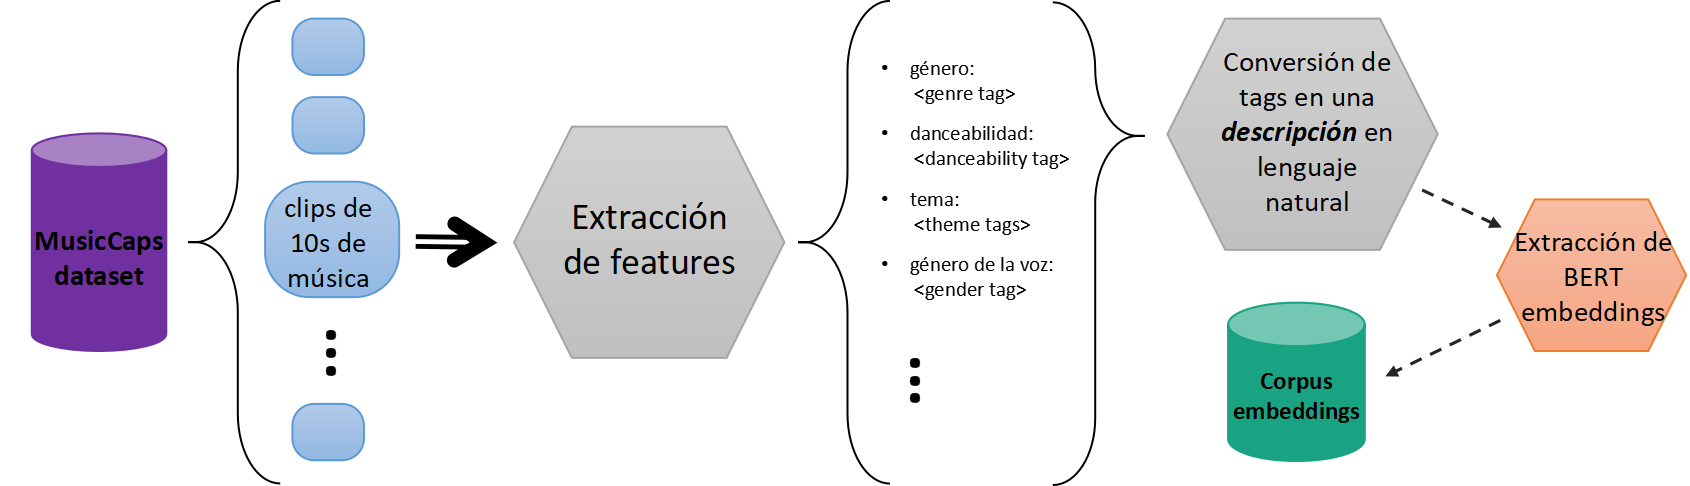
\includegraphics[width=\textwidth]{Graphics/corpus_embeddings.png}
	\caption{Diseño propuesto.} 
    \label{fig:corpus_embeddings}
\end{figure}

En el apartado de recuperación de información, el sistema consiste en recopilar la consulta del usuario, generar el vector de embedding con SBERT y encontrar las canciones más similares comparando el vector con el corpus de embeddings, utilizando similitud de coseno. En la imagen \ref{fig:sri_design} se observa el diseño del SRI. % TODO cite other BERT stuff that does this

\begin{figure}[h!]
	\centering
	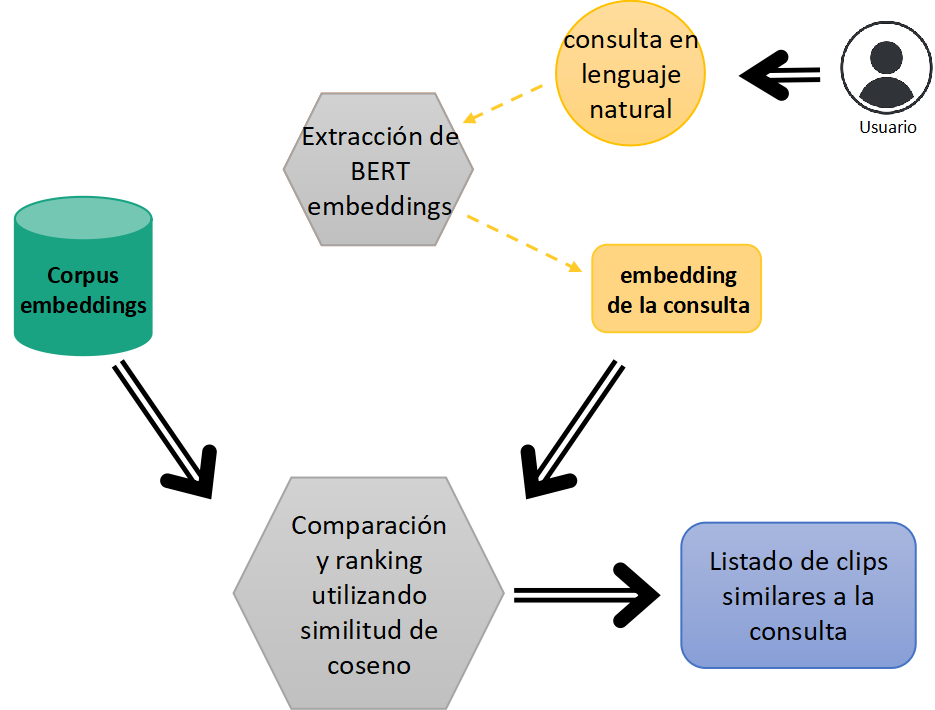
\includegraphics[width=0.6\textwidth]{Graphics/SRI.png}
	\caption{Sistema de recuperación utilizando \textit{Sentence BERT embeddings}.} 
    \label{fig:sri_design}
\end{figure}

\section{Dataset}
\label{sec:dataset}

Para establecer un baseline de la eficacia del prototipo a implementar es necesario evaluarlo con las métricas usuales en SRI y preferentemente en el mismo conjunto de datos que otros trabajos en el tema. 

\textit{Contrastive Audio-Language Learning for Music} \cite{Manco2022ContrastiveAL} entrenaron y evaluaron su modelo de recuperación en un \textit{dataset} de 250 mil pares (audio, texto) creado a partir de una biblioteca de música en producción. Pero no se encuentra disponible públicamente para utilizarlo y comparar justamente los resultados.

La evaluación de recuperación de música a partir de consultas textuales de \textit{MuLan: A Joint Embedding of Music Audio and Natural Language} \cite{Huang2022MuLanAJ} fue una colección patentada de 7,000 listas de reproducción curadas por expertos. Que tampoco fue encontrada públicamente.

Dado la idea mencionada en la sección \ref{subsec:music_captioning}, decidimos encontrar un \textit{dataset} de \textit{captioning}. Sin embargo la mayor parte de los datasets de captioning utilizados en la literatura son privados. Finalmente decidimos utilizar MusicCaps, que fue liberado públicamente en \cite{Agostinelli2023MusicLMGM}, una investigación apenas de este año. 

En \textit{HuggingFace} \cite{huggFaceMusicCaps} aparece una descripción del \textit{dataset}, el .csv y en \href{https://github.com/nateraw/download-musiccaps-dataset}{este link de github} hay un \textit{script} para descargar los clips de YouTube. MusicCaps contiene 5,521 clips de 10 segundos, extraídos de AudioSet \cite{Gemmeke2017AudioSA}. Por cuestiones de inaccesibilidad a la cantidad suficiente de internet, para esta investigación utilizamos un subconjunto de clips, lo que no causa ningún problema dado que no necesitamos una cantidad de datos específica con que entrenar. Cada clip contiene una lista de 'aspectos' en inglés y una descripción de texto libre escrita por músicos. Una lista de aspectos es, por ejemplo, "\textit{pop, tinny wide hi hats, mellow piano melody, high pitched female vocal melody, sustained pulsating synth lead}". Mientras que la descripción consta de varias oraciones sobre la música, por ejemplo, " \textit{A low sounding male voice is rapping over a fast paced drums playing a reggaeton beat along with a bass. Something like a guitar is playing the melody along. This recording is of poor audio-quality. In the background a laughter can be noticed. This song may be playing in a bar.} "

La escasez de datasets en MIR es un gran obstáculo en el desarrollo del campo. Se debe, en parte, a que a diferencia de otros tipos de multimedia, la música tiende a tener \textit{copyright} lo que impide crear conjuntos de datos con ejemplos representativos, que además sean lo suficientemente grandes para ser útiles en las arquitecturas de redes neuronales utilizadas en el presente aprender en el campo de texto, o imágenes, por ejemlo. Esto ha implicado que varias investigaciones recientes, incluyendo la nuestra, decidan apoyarse en las capacidades de transferencia de conocimiento que poseen los modelos de lenguaje, como fue explicado en la sección \ref{subsec:learning_lang_superv}, para tareas en MIR que incluyan trabajo con texto.

\section{Detalles de implementación}
\label{sec:implementation}

% El sistema de validación de modelos para un VRP específico cuenta con cuatro componentes descritos en el capítulo anterior. En este capítulo se presentan las abstracciones realizadas para llevar a cabo la implementación de cada una de las componentes. Además, se describen los detalles de la implementación realizada en este trabajo. En la sección \ref{sec:def} se describe la manera propuesta para definir un VRP. Posteriormente, en las secciones \ref{sec:highSol}, \ref{sec:lowSol} y \ref{sec:func} se muestran los detalles de implementación de los primeros tres componentes del sistema: el generador de soluciones de alto nivel, el generador de soluciones de bajo nivel y el generador de funciones, respectivamente. Por último, se presenta el pseudocódigo general seguido en la evalución del modelo y la implementación llevada a cabo en el trabajo.

% A continuación se muestra la manera de definir un VRP para poder evaluar el modelo correspondiente.

% \section{Definición de un VRP} \label{sec:def}
% Las características abstractas se definieron, en la sección \ref{sec:inputs}, como la manera propuesta en este trabajo para describir un problema de enrutamiento de vehículos. Cada una de las características se representa mediante una clase sin campos y que no hereda de ninguna otra.

% A modo de ejemplo, se definen las clases {\tt visit-client-at-least-once}, {\tt visit-client-at-most-once}, {\tt dont-overload-vehicles} y {\tt begin-end-in-\\depot}. Con estas clases creadas es posible definir el CVRP como una clase que hereda de todas las características que lo definen. El código \ref{alg:cvrp} muestra lo anterior.

% \begin{figure}[h!] 
% \begin{lstlisting}
% (defclass cvrp (dont-overload-vehicles
%                 begin-end-in-depot
%                 visit-client-at-most-once
%                 visit-client-at-least-once) ())
% \end{lstlisting}
% 	\caption{Definición del CVRP a partir de las características abstractas.}  \label{alg:cvrp}
% \end{figure}

% Para simular los elementos del conjunto $B_A$ mostrado en la sección \ref{sec:inputs} se define, para cada característica abstracta, al menos una {\it característica opuesta} que represente el comportamiento contrario a dicha característica abstracta. Por ejemplo, para las características mostradas con anterioridad, se implementan las clases {\tt dont-visit-all-clients}, {\tt visit-client-more-\\than-once}, {\tt overload-vehicles} y {\tt begin-end-anywhere}.

% Una característica abstracta puede tener varias características opuestas que definan distintas maneras de incumplirlas. Por ejemplo, para no satisfacer la característica de comenzar y terminar una ruta en el depósito central, se puede no empezar en el depósito, no terminar en él o ambas opciones. Estos comportamientos pueden ser modelados, cada uno, por distintas clases.

% Para construir el conjunto $B_A$, es necesario conocer para cada característica abstracta, las características opuestas que le corresponden. Para ello se tiene la función {\tt opposite-characteristics} que dada una característica abstracta, devuelve el conjunto de características opuestas. Por ejemplo, cuando se evalúa esta función con el nombre de la clase {\tt dont-overload-\\vehicles}, se obtendría como resultado el nombre de la clase {\tt overload-ve-\\hicles}.

% Una vez definido el problema para el cual se desea validar un modelo y el conjunto de características opuestas, es posible generar las soluciones de alto nivel como muestra la siguiente sección.

% \section{Generación de soluciones de alto nivel} \label{sec:highSol}
% El generador de soluciones de alto nivel crea soluciones a partir de un conjunto de requerimientos. Cada elemento de este conjunto es una combinación de características abstractas y opuestas que representa un elemento de $B_A$. Para generar las soluciones de manera que cumplan cada una de las características, se define una función genérica {\tt generate-solution}. Esta función recibe el requerimiento y una solución e instancia de problema vacías. Por cada característica presente en el requerimiento se modifica el elemento en la solución o el problema a la que esa característica afecte. De esta manera, una vez se termine de recorrer todos los elementos que conforman el requerimiento se tendrá una solución y un problema que lo satisfagan.

% Por ejemplo, la clase {\tt cvrp}, mostrada en \ref{alg:cvrp}, define un requerimiento: el de las soluciones factibles para el CVRP. Con esta clase, la función {\tt generate-solution} recorrería cada característica en {\it determinado orden}. Supongamos que para ese ejemplo el orden establecido es de la característica final a la primera. En este caso, {\tt visit-client-at-least-once} añade el conjunto de clientes al problema y luego crea rutas en la solución donde todos los clientes son visitados al menos una vez. Luego, {\tt visit-client-at-\\most-once} verifica que en el conjunto de rutas ya creado se visite una única vez a cada cliente y, de no ser así, elimine a los clientes repetidos. Con la característica {\tt begin-end-in-depot} se añade el depósito al inicio y al final de cada una de las rutas. Finalmente, {\tt dont-overload-vehicles} define una capacidad en el problema que impida que las rutas ya definidas sean visitadas por vehículos sobrecargados, por ejemplo, tomando como la capacidad la suma de las demandas de todos los clientes.

% A partir del ejemplo se puede notar que el orden en el que se definan las características es importante a la hora de construir las soluciones. Si se hubiera analizado primero la característica {\tt dont-overload-vehicles}, esta, además de trazar una estrategia para definir la capacidad de los vehículos, tendría que construir el conjunto de clientes y las rutas para garantizar que se cumpla la restricción de capacidad. Esto complicaría la construcción de la solución en las características siguientes pues habría que verificar un mayor número de condiciones. Por ejemplo, al analizar {\tt dont-overload-vehi-\\cles} primero, {\tt visit-client-at-most-once} debe controlar que las rutas creadas visiten a lo sumo una vez a cada cliente y, de no cumplirse, modificarlas para que satisfagan esta restricción. De suceder esto, las restricciones de capacidad tienen que ser verificadas de nuevo.

% La decisión del orden correcto para definir las características de un problema depende de la implementación de la función genérica {\tt generate-so-\\lution} para cada característica. En el caso de este trabajo, el orden correcto para el CVRP es el definido en el código \ref{alg:cvrp}. A continuación se presentan los detalles de la implementación propuesta para este trabajo.

% \subsection{Implementación de la función {\tt generate-solution}}
% La implementación de la función {\tt generate-solution} se realizó haciendo uso de las funcionalidades del lenguaje Common Lisp descritas en la sección \ref{sec:lisp}. La definición de la función genérica {\tt generate-solution} se muestra en la figura \ref{alg:gsGeneric}.

% \begin{figure}[h!] 
% \begin{lstlisting}
% (defgeneric generate-solution (condition
%                                solution
%                                problem
%                                log))
% \end{lstlisting}
% 	\caption{Definición de la función genérica {\tt generate-solution}.}  \label{alg:gsGeneric}
% \end{figure}

% La función recibe una solución ({\tt solution}) y un problema ({\tt problem}) vacío que se modificarán a medida que se analicen las características definidas en la condición ({\tt condition}). En cada una de las implementaciones de la función genérica, el parámetro {\tt condition} se especializa en una característica distinta (ya sea abstracta u opuesta). En el parámetro {\tt log} se registran los pasos llevados a cabo para construir la solución.

% La manera de definir una condición es a través de una clase que herede de las características que debe cumplir la solución y el problema generado como se observa en la figura \ref{alg:cvrp}. Esta forma permite que al especificar {\tt :after} luego de la definición de los métodos para cada característica, se invoquen todas las implementaciones de la función genérica {\tt generate-function}. Como los métodos {\tt :after} se ejecutan de menos a más específicos, el orden de ejecución sería de la última característica a la primera. En el caso del ejemplo \ref{alg:cvrp} se ejecuta en el orden inverso de la lista de los ancestros, es decir, primero el método donde {\tt condition} se haya especializado en {\tt visit-client-at-least-once} y por último el correspondiente a la clase {\tt dont-overload-vehicles}.

% Por ejemplo, la definición del método para generar soluciones que cumplan con la característica {\tt visit-client-at-least-once} se muestra en la figura \ref{alg:gsMethod:vcalo}. En el cuerpo de dicho método se generan una cantidad aleatoria de clientes y se selecciona el número de rutas $K$. Para construir dichas rutas se divide una permutación del conjunto de clientes en $K$ conjuntos que representan las rutas. Las demandas de cada cliente son también elegidas de manera aleatoria. De esta forma se garantiza que cada cliente sea visitado al menos una vez.

% \begin{figure}[h!] 
% \begin{lstlisting}
% (defgeneric generate-solution :after
%             ((condition visit-client-at-least-once)
%              solution
%              (problem cvrp-problem)
%              log)
%  ;; generar las soluciones
%  )
% \end{lstlisting}
% 	\caption{Definición del método {\tt generate-solution} para la característica {\tt visit-client-at-least-once}.}  \label{alg:gsMethod:vcalo}
% \end{figure}

% Como la definición de un método primario es obligatoria, se implementó uno con el cuerpo vacío.

% Una vez construidas las soluciones de alto nivel y las instancias del problema, es posible generar las soluciones de bajo nivel. La sección siguiente describe los elementos necesarios para implementar este componente.

% \section{Generación de soluciones de bajo nivel} \label{sec:lowSol}
% El generador de soluciones de bajo nivel transforma las soluciones de alto nivel en conjuntos de variables, parámetros y conjuntos presentes en el modelo.

% Para construir el conjunto de variables es necesario conocer, además de la solución de alto nivel, el tipo de formulación con la que se modeló el problema. De esta manera, cuando se valide el modelo por flujo de mercancías del CVRP se podrán generar las variables correctas $x_{ij}$ y $y_{ij}$. Sin embargo, en la sección \ref{subsec:modelTypes} se presentaron formulaciones que, en dependencia del problema, podían agregar nuevas variables. Por esta razón, cuando se quiera validar un modelo es necesario implementar la transformación de la solución a las variables involucradas en ese modelo en específico.

% El conjunto de parámetros y conjuntos es dependiente del problema. Además, un mismo problema puede ser modelado utilizando conjuntos de parámetros distintos. Al igual que con la generación del conjunto de variables, los conjuntos de parámetros y de conjuntos debe implementarse para cada modelo específico. Con esto se garantiza que la transformación genere exactamente los mismos conjuntos que aparecen en el modelo.


% La generación de las soluciones de bajo nivel puede realizarse en una misma función {\tt generate-low-level-solution}. Sin embargo, la implementación propuesta en este trabajo cuenta con dos funciones {\tt generate-varia-\\bles} y {\tt generate-param-set-values} donde se generan el conjunto de variables y el conjunto de parámetros y conjuntos, respectivamente. A continuación se muestran los detalles de la implementación propuesta para estas funciones.

% \subsection{Implementación de la función {\tt generate-variables}}
% La generación del conjunto de variables se realiza a través de la función genérica {\tt generate-variables} definida en la figura \ref{alg:gvGeneric}

% \begin{figure}[h!] 
% \begin{lstlisting}
% (defgeneric generate-variables (solution
%                                 problem
%                                 model-type))
% \end{lstlisting}
% 	\caption{Definición de la función genérica {\tt generate-variables}.}  \label{alg:gvGeneric}
% \end{figure}

% Las entradas {\tt solution} y {\tt problem} representan la solución y el problema creados en el generador de soluciones de alto nivel.

% El tipo de modelo ({\tt model-type}) se representa mediante una clase para cada formulación posible. Por esta razón, se implementaron las clases {\tt commodity-flow}, {\tt two-index-vehicle-flow} y {\tt three-index-vehicle-flow} para las formulaciones por flujo de mercancías, flujo de vehículos de dos índices y flujo de vehículos de tres índices, respectivamente. La entrada {\tt model-type} se especializa en cada una de las clases mencionadas.

% Esta función asigna los valores correctos para cada una de las variables presentes en el problema a partir de la solución ya generada.

% Por ejemplo, para el modelo por flujo de mercancía del CVRP se conoce que son necesarias las variables $x_{ij}$ y $y_{ij}$ que representan el paso y la capacidad residual de un vehículo que va del nodo $i$ al nodo $j$, respectivamente. En este caso, la función {\tt generate-variables} recorre las rutas definidas en la solución y le asigna el valor 1 a cada variable $x_{ij}$ si se visita al cliente $j$ después del cliente $i$. Además, a la capacidad $C$ del vehículo le resta la demanda del cliente $i$ cuando se pasa al cliente $j$ y le asigna este valor a la variable $y_{ij}$. A $y_{ji}$ le asigna el resultado de la operación $C - y_{ij}$. Para la solución \ref{fig:probSolEj} de la página \pageref{fig:varEj}, las variables generadas se muestran en la figura \ref{fig:varEj} que aparece en la misma página. El encabezado que tendría la implementación de la función genérica {\tt generate-variables} para el ejemplo se muestra en la figura \ref{alg:gvMethod:cf}.

% \begin{figure}[h!] 
% \begin{lstlisting}
% (defgeneric generate-variables
%             (solution
%              (problem cvrp-problem)
%              (model-type commodity-flow))
%  ;; generar variables
%  )
% \end{lstlisting}
% 	\caption{Encabezado del método {\tt generate-variables} para el modelo por flujo de mercancías del CVRP.}  \label{alg:gvMethod:cf}
% \end{figure}

% \subsection{Implementación de la función {\tt generate-param-set-values}} \label{subsec:gpsv}
% Los conjuntos de parámetros y conjuntos solo depende de la solución y problema creados en el generador de soluciones de alto nivel. Por esta razón, la función genérica {\tt generate-param-set-values} definida en la figura \ref{alg:gpsGeneric} solo tiene dos entradas: {\tt solution} y {\tt problem}. La primera representa la solución y la segunda, la instancia de problema.

% \begin{figure}[h!] 
% \begin{lstlisting}
% (defgeneric generate-param-set-values (solution
%                                        problem))
% \end{lstlisting}
% 	\caption{Definición de la función genérica {\tt generate-param-set-values}.} \label{alg:gpsGeneric}
% \end{figure}

% Con el conjunto de parámetros y conjuntos generados, es posible definir las funciones que representan cada una de las restricciones del problema y en las que se evaluará el conjunto de variables. En la siguiente sección se muestran los elementos tenidos en cuenta para la implementación del generador de funciones.

% Para el CVRP se necesitan los parámetros $C$, $d$, $K$ que representan la capacidad de los vehículos, la demanda de cada cliente y la cantidad de vehículos, respectivamente. Además, se tiene el conjunto $V$ de clientes. La función {\tt generate-param-set-values} asigna los valores adecuados para cada uno de estos parámetros y conjuntos a partir de la solución y el problema. Para el ejemplo de solución y problema de la figura \ref{fig:probSolEj2} se generarían los conjuntos mostrados en la figura \ref{fig:paramSetEj}.

% \begin{figure}[h!]
% 	\begin{minipage}{0.45\textwidth}
% 		{\bf Problema}
		
% 		{\tt cantidad de clientes: 3\\capacidad: 3\\depósito: 0\\demandas: $\{1, 2, 1\}$}
% 	\end{minipage}
% 	\hfill
% 	\begin{minipage}{0.45\textwidth}
% 		{\bf Solución}
		
% 		{\tt rutas: $\{0, 1, 2, 0\}$ y $\{0, 3, 0\}$}
% 	\end{minipage}
% 	\caption{Problema y solución generada para el requerimiento $(\{1, 2, 3\}, \{\})$.} \label{fig:probSolEj2}
% \end{figure}

% \begin{figure}[h!]
% 	\centering
% 	\begin{minipage}{0.45\textwidth}
% 		\begin{center}
% 			$n = 3$
			
% 			$K = 2$
			
% 			$C = 3$
			
% 			$d = (1,\ 2,\ 3)$
% 		\end{center}
% 	\end{minipage}
% 	\hfill \begin{minipage}{0.45\textwidth}
% 		$V = \{0,\ 1,\ 2,\ 3,\ 4\}$
% 	\end{minipage}
% 	\caption{Conjunto de parámetros $p_i$ (a la izquierda) y conjunto de instancias de los conjuntos $c_i$ (a la derecha) para la solución y problema de la figura \ref{fig:probSolEj2}}
% 	\label{fig:paramSetEj}
% \end{figure}

% \section{Generación de funciones} \label{sec:func}
% La generación de funciones se realiza utilizando el Árbol de Sintaxis Abstracta (AST)\footnote{Los Árboles de Sintaxis Abstracta (AST) representan jerárquicamente, mediante un árbol, la estructura sintáctica abstracta o simplificada de un programa escrito en un lenguaje de programación.} que se obtiene a partir del modelo descrito en algún AML. En este trabajo se usa LMML. Con en el AST se puede organizar las operaciones que se realizan en cada restricción.

% Por ejemplo, si se tiene la restricción $s.a\ x_{ij} \geq 0 \ \ \forall i, j \in V$, se obtiene el AST mostrado en la figura \ref{fig:ast}.

% \begin{figure}[h!]
% 	\centering
% 	\includegraphics[width=0.75\textwidth]{MainMatter/images/ast.png}
% 	\caption{AST obtenido a partir de la restricción $s.a\ x_{ij} \geq 0 \ \ \forall i, j \in V$.} \label{fig:ast}
%       \end{figure}

% A partir del AST se pueden realizar recorridos donde, en dependencia del nodo en el que se encuentre, se genere el fragmento de código correspondiente a la función. Para el ejemplo de la figura \ref{fig:ast} se puede realizar un recorrido donde, cuando se encuentre el nodo $s.a.$ se cree el encabezamiento de la función que se quiere generar. A continuación, se puede recorrer cada una de las ramas de izquierda a derecha para generar el código de la operación que se debe realizar y de los índices. Los códigos generados son dependientes del lenguaje en el que se desee realizar la validación.

% Como las funciones reciben las variables del modelo como entrada, es necesario conocer previamente qué variables se definen en él. Para ello se realiza un recorrido por el AST del modelo que reúna todas las variables. Este recorrido se lleva a cabo en la función {\tt collect-variables}.

% Para la transformación de las restricciones se define una función {\tt gene-\\rate-functions} encargada de recorrer el AST del modelo y crear, por cada restricción, una función cuyas entradas sean cada una de las variables del modelo recolectadas previamente. Las funciones, al no recibir los parámetros y conjuntos del modelo, deben sustituir los identificadores de los mismos por los valores correspondientes. Dichos valores se obtienen en el generador de soluciones de bajo nivel.

% El trabajo propone una implementación de las funciones {\tt collect-va-\\riables} y {\tt generate-functions} que hace uso de las funcionalidades de LMML. A continuación se describen los detalles de la implementación de las funciones {\tt collect-variables} y {\tt generate-functions}.

% \subsection{Implementación de la función {\tt collect-variables}}
% LMML estructura el modelo a partir de clases que representan las operaciones que definen las restricciones y función objetivo de un modelo. De esta forma, cuando se escribe un modelo en LMML, la estructura que se obtiene es el AST del mismo.

% El recorrido que permite recolectar todas las variables del modelo se implementa en la función genérica {\tt collect-variables}. La definición de esta se muestra en la figura \ref{alg:cvGeneric}.

% \begin{figure}[h!] 
% \begin{lstlisting}
% (defgeneric collect-variables (model-instruction
%                                model))
% \end{lstlisting}
% 	\caption{Definición de la función genérica {\tt collect-variables}.} \label{alg:cvGeneric}
% \end{figure}

% La entrada {\tt model-instruction} se especializa en cada una de las clases que pueden encontrarse en el AST, solo guardando el nombre de las variables definidas cuando se encuentra con el nodo de {\tt variable-declaration}. La función devuelve una lista de los nombres de todas las variables declaradas en el modelo. Con esta lista es posible generar las funciones correspondientes a cada una de las restricciones del modelo como se muestra en la sección siguiente.

% \subsection{Implementación de la función {\tt generate-functions}}
% Para generar las funciones se define la función genérica {\tt generate-\\functions} como se muestra en la figura \ref{alg:gfGeneric}.

% \begin{figure}[h!]
% \begin{lstlisting}
% (defgeneric generate-functions (ast-node
%                                 param-set-values
%                                 variables))
% \end{lstlisting}
% 	\caption{Definición de la función genérica {\tt generate-functions}.} \label{alg:gfGeneric}
% \end{figure}

% La entrada ({\tt ast-node}), que representa el nodo del AST que se esté analizando en el momento, se especializa en las distintas clases definidas en LMML. En cada uno se genera el fragmento de código de Common Lisp que permite obtener funciones evaluables.

% Cuando en el recorrido se encuentre una referencia a un parámetro o conjunto, se verifica que estén en la lista {\tt param-set-values} y se sustituye su nombre por el valor correspondiente. Como puede deducirse, es importante que el nombre con el que se definen los parámetros y conjuntos en el modelo coincida con los nombres recogidos en la lista. Actualmente, esto solo se garantiza mediante la implementación manual de la función {\tt generate-param-set-values} mostrada en la sección \ref{subsec:gpsv}.

% El conjunto de nombres de variables ({\tt variables}) se utiliza para definir la entrada de cada función.

% Para el AST visto en la figura \ref{fig:ast}, la función {\tt generate-functions} generaría la función matemática siguiente:

% $$
% f(x) = \left\{\begin{array}{cl}
% 				1 & si\ x_{ij} \geq 0  \ \ \forall i, j \in V\\
% 				0 & en\ otro\ caso
% 			  \end{array}\right.
% $$

% Con todas estas funciones definidas, es posible pasar a la evaluación del modelo. La siguiente sección describe el algoritmo con el que evaluar un modelo de entrada para un VRP específico.

% \section{Evaluación del modelo} \label{sec:eval}
% En la evaluación del modelo se combinan todas las funciones vistas hasta el momento en las secciones anteriores y se implementa la estrategia descrita en el capítulo \ref{chap:system} como se muestra en el pseudocódigo \ref{alg:mePseudocode}.

% \begin{algorithm}[htb]
% 	\caption{Algoritmo propuesto para la validación automática de un modelo para VRP}\label{alg:mePseudocode}
% 	\SetAlgoLined
% 	\KwData{Características abstractas $A$ del VRP y modelo $M$}
% 	\KwResult{Verdadero si el modelo parece correcto; falso si no}
% 	\LinesNumbered
% 	\SetAlgoVlined
% 	$B_A = \{(C_i, C_i^c) | C_i \subseteq A\ \ \forall i = \overline{1, 2^{|A|}}\}$\;
% 	\For{$(C_i, C_i^c) \in B_A$}{
% 		\For{$k = 1, 2, \dots, K$}{
% 			$S_{ik}, P_{ik} = generate\_solution(C_i, C_i^c)$\;
% 			$v_{ik}, p_{ik}, c_{ik} = generate\_low\_level\_solution(S_{ik}, P_{ik})$\;
% 			$v_{name} = collect\_variables(M)$\;
% 			$f_{ik} = generate\_functions(M, p_{ik}, c_{ik}, v_{name})$\;
% 			\If{$f(v_{ik})\ \ \forall f \in f_{ik}$}{
% 				$continue$\;}
% 			\Else{\Return Falso, ($S_{ik}, P_{ik}$)\;}
% 		}
% 	}
% 	\Return Verdadero\;
% \end{algorithm}

% En este trabajo se implementó la evaluación del modelo en la función {\tt evaluate-model} cuya definición se muestra en la figura \ref{alg:emFunction}.

% \begin{figure}[h!]
% \begin{lstlisting}
% (defgeneric evaluate-model (problem
%                             model))
% \end{lstlisting}
% 	\caption{Definición de la función {\tt evaluate-model}.} \label{alg:emFunction}
% \end{figure}

% La entrada {\tt problem} representa el problema descrito mediante las clases que representan sus características abstractas, mientras que {\tt model} es la especificación del modelo que se debe evaluar, escrito en LMML. El problema se debe definir como se muestra en el código \ref{alg:cvrp}.

% Además de conocer los detalles de la implementación del sistema propuesto en este trabajo, es importante presentar la manera en la que se pueden incorporar nuevos problemas y modelos. En la próxima sección se ilustran los recursos del sistema para realizarlo.

% \section{Extensibilidad}

% En esta tesis solo se implementó la validación del modelo de flujo de mercancías del CVRP. Sin embargo, cuenta con los recursos necesarios para que pueda ser extendido a otros problemas y modelos, como se presenta en esta sección. Inicialmente se ilustrará la manera de definir nuevos problemas y, posteriormente, la manera de incorporar nuevos modelos.

% \subsection{Definición de nuevos problemas}
% En este trabajo se propuso la definición de un VRP a partir de un conjunto de características abstractas. Actualmente, el sistema cuenta con la implementación de las características del CVRP. Sin embargo, es posible la incorporación de nuevos problemas.

% Como se comentó en la sección \ref{sec:def}, cada característica abstracta de un problema se representa mediante una clase que no cuenta con campos ni ancestros. Para cada característica debe existir, al menos, la implementación de una característica opuesta.

% Por ejemplo, si se quisiera añadir la característica del VRPB de visitar a todos los clientes cuya demanda debe ser satisfecha antes de los clientes a los que se le debe recoger una cantidad, entonces es necesario crear la clase mostrada en el código \ref{alg:vrpbCA}.

% \begin{figure}[h!] 
% \begin{lstlisting}
% (defclass linehaul-before-backhaul () ())
% \end{lstlisting}
% 	\caption{Definición de una nueva característica abstracta para el VRPB.} \label{alg:vrpbCA}
% \end{figure}

% Además, se debe definir al menos una característica opuesta como se ilustra en el código \ref{alg:vrpbCO}.

% \begin{figure}[h!] 
% \begin{lstlisting}
% (defclass not-linehaul-before-backhaul () ())
% \end{lstlisting}
% 	\caption{Definición de una nueva característica abstracta para el VRPB.} \label{alg:vrpbCO}
% \end{figure}

% Es importante aclarar que en este, como en muchos otros casos, es posible definir más de una manera de incumplir la característica abstracta y, para ello, pueden crearse varias clases que representen cada uno de esos comportamientos. Por ejemplo, para incumplir la característica definida en \ref{alg:vrpbCA}, puede intercalarse cada tipo de cliente o puede invertirse el orden, es decir, primero los clientes a los que hay que recogerle algún producto y después los clientes a los que hay que llevarle alguna mercancía.

% Para conocer qué características opuestas le corresponden a determinada característica abstracta, es necesario implementar la función {\tt opposite-\\characteristics}.

% Con las características abstractas y opuestas bien definidas, es posible pasar a realizar la generación de las  soluciones e instancias de problemas. Esto se realiza especializando el parámetro {\tt condition} de la función genérica {\tt generate-solution} en la clase correspondiente a la característica que se quiera cumplir (ya sea abstracta u opuesta) y modificando en el cuerpo del método la solución y el problema según sea pertinente.

% Una vez se define una característica y la manera de generar soluciones e instancias de problemas a partir de ella, esta puede ser usada en la definición de cualquier problema cuya solución deba satisfacer dicha característica.

% A continuación se muestra la manera de definir un nuevo modelo.

% \subsection{Definición de nuevos modelos}
% Para definir un nuevo modelo se debe conocer el tipo de formulación que utiliza y las variables, parámetros y conjuntos que relaciona.

% Cada tipo de formulación se define mediante una clase sin campos ni ancestros. Actualmente, el sistema cuenta con la implementación de los tres tipos de modelo presentados en la sección \ref{subsec:modelTypes}.

% Para definir los valores del conjunto de variables a partir de la solución y el problema, se debe especializar el parámetro de {\tt model-type} en la función genérica {\tt generate-variables}. En el cuerpo del método debe implementarse la manera de obtener el conjunto adecuado de variables. Por ejemplo, para el modelo por flujo de vehículos de tres índices del VRPTW, se debe definir la función mostrada en el código \ref{alg:vrptwGV}.

% \begin{figure}[h!] 
% \begin{lstlisting}
% (defmethod generate-variables
%     (solution
%      (problem vrptw-problem)
%      (model-type three-index-vehicle-flow))
%     ;; instrucciones para generar variables
%     )
% \end{lstlisting}
% 	\caption{Definición del método para obtener los valores de las variables $x_{ijk}$ y $w_{ik}$ para el modelo de flujo de vehículos de tres índices del VRPTW.} \label{alg:vrptwGV}
% \end{figure}

% Como el conjunto de parámetros y conjuntos depende del problema y la modelación que se realice, cuando se define un nuevo modelo se debe implementar la función {\tt generate-param-set-values}. En el cuerpo de la misma deben asignarse los valores adecuados para los parámetros y conjuntos del nuevo modelo y problema.

% Al definirse el modelo en LMML, la generación de funciones se realiza de manera completamente automática, por lo que no es necesario realizar ninguna modificación en este componente.

% En este capítulo se describieron los detalles de implementación y la extensibilidad del sistema de validación de modelos para un VRP propuesto. En el próximo capítulo se presentarán los resultados obtenidos cuando se probó la herramienta en el modelo de CVRP por flujo de mercancías definido en Toth y Vigo \cite{toth@vrp}.

% \chapter{Validación del modelo por flujo de mercancías del CVRP}
% \label{chap:results}

% El CVRP es la variante más sencilla y estudiada de los VRP \cite{toth@vrp}. Para describirlo se han definido numerosos modelos mediante distintos tipos de formulaciones. En el capítulo \ref{chap:preliminaries} se mostraron dos de estos modelos: uno con flujo de vehículos de dos índices y otro con flujo de mercancías. En el libro de Toth y Vigo \cite{toth@vrp} se presenta un modelo por flujo de mercancía distinto al presentado en este trabajo. A continuación se muestra el modelo propuesto por Toth y Vigo:

% $$
% \min \sum_{(i, j) \in A} c_{ij} x_{ij}
% $$
% \begin{eqnarray}
% s.a \displaystyle{\sum_{j \in V} (y_{ji} - y_{ij})} & = & 2 d_i \ \ \forall i \in V / \{0, n + 1\}\\
% \displaystyle{\sum_{j \in V / \{0, n + 1\}} y_{0j}} & = & d(V / \{0, n + 1\})\\
% \displaystyle{\sum_{j \in V / \{0, n + 1\}} y_{j0}} & = & KC - d(V / \{0, n + 1\})\\
% \displaystyle{\sum_{j \in V / \{0, n + 1\}} y_{n + 1 j}} & = & KC\\
% y_{ij} + y_{ji} & = & Cx_{ij} \ \ \forall (i, j) \in A\\
% \displaystyle{\sum_{j \in V} (x_{ij} + x_{ji})} & = & 2 \ \ \forall i \in V / \{0, n + 1\}\\
% y_{ij} & \ge & 0 \ \ \forall (i, j) \in A\\
% x_{ij} & \in & {0, 1} \ \ \forall (i, j) \in A
% \end{eqnarray}

% En este capítulo se realizará la validación de este modelo con el sistema implementado. En las secciones \ref{sec:systemInput} y \ref{sec:systemOutput} se presentan la entrada y la salida del sistema, respectivamente. Por último, en la sección \ref{sec:results} se describe la interpretación de estos resultados.

% \section{Entradas del sistema}\label{sec:systemInput}
% Para probar el sistema se realizaron varias ejecuciones con distintos valores de $k$. Las pruebas realizadas con el sistema para validar el modelo por flujo de mercancías del CVRP utilizaron valores de $k$ iguales a 1 y a 10.

% La implementación del modelo en LMML se muestra en el código \ref{alg:cvrpLMML} de la página \pageref{alg:cvrpLMML}.

% \begin{figure}[h!] 
% \begin{lstlisting}[basicstyle=\bfseries\ttfamily\footnotesize]
% (defparameter
%     cvrp-model
%     (problem "cvrp"
%              (set V)
%              (set I)
%              (param c :domain {V V})
%              (param d :domain {V})
%              (param n)
%              (param P)
%              (param K)
%              (param M)
%              (binary-variable x :domain {V V})
%              (variable        y :domain {V V})
%              (minimize (sum (a in V)
%                          (sum (b in V)
%                              x[a b] * c[a b])))
%              (s.t. (sum (b in V)
%                        y[b a] - y[a b]) = 2 * d[a]
%                    (forall a in I))
%              (s.t. (sum (b in I) y[0 b]) = M)
%              (s.t. (sum (b in I) y[b 0]) = K * P - M)
%              (s.t. (sum (b in I) y[n + 1 b]) = K * P)
%              (s.t. y[a b] + y[b a] = P * x[a b]
%                    (forall a in V)
%                    (forall b in V))
%              (s.t. (sum (b in V)  x[a b] + x[b a]) = 2
%                    (forall a in I))))
% \end{lstlisting}
% 	\caption{Definición del modelo por flujo de mercancías del CVRP en LMML.}  \label{alg:cvrpLMML}
% \end{figure}

% Otra de las entradas del sistema es la definición del problema mediante las características abstractas. Para el CVRP, las manera de definirlo se muestra en el código \ref{alg:cvrp2}.

% \begin{figure}[h!] 
% \begin{lstlisting}
% (defclass cvrp (dont-overload-vehicles
%                 begin-end-in-depot
%                 visit-client-at-most-once
%                 visit-client-at-least-once) ())
% \end{lstlisting}
% 	\caption{Definición del CVRP a partir de las características abstractas.}  \label{alg:cvrp2}
% \end{figure}

% Con los argumentos de la función {\tt evaluate-model} definidos, es posible pasar a la evaluación del sistema cuya salida se explica en la sección siguiente.

% \section{Salida del sistema}\label{sec:systemOutput}
% Con la salida del sistema es posible conocer qué pruebas resultaron exitosas y cuáles fallaron. Para las pruebas fallidas se muestran ejemplos de soluciones (factibles e infactibles en dependencia del requerimiento) donde las restricciones del modelo resultaron incorrectas.

% Al validar el modelo presentado en la página \pageref{alg:cvrpLMML} con la función {\tt evaluate\\-model} el resultado para cada prueba en la que se generan soluciones infactibles es satisfactorio, pues al menos una restricción se incumple. Sin embargo, al evaluar soluciones factibles en las restricciones del modelo, la prueba falla.

% Para cada una de las $k$ soluciones factibles generadas ($k = 1$ y $k = 10$), la restricción (4.5) falla. Uno de los ejemplos de solución devuelto por el sistema, que incumple dichas restricción, se muestra en la figura \ref{fig:wrongSolEj}.

% \begin{figure}[h!]
% 	\begin{minipage}{0.45\textwidth}
% 		{\bf Problema}
		
% 		{\tt cantidad de clientes: 3\\capacidad: 18\\depósito: 0\\demandas: $\{6, 9, 3\}$}
% 	\end{minipage}
% 	\hfill
% 	\begin{minipage}{0.45\textwidth}
% 		{\bf Solución}
		
% 		{\tt rutas: $\{0, 3, 0\}$ y $\{0, 1, 2, 0\}$}
% 	\end{minipage}
% 	\caption{Problema y solución de ejemplo generada por el sistema que falla una de las pruebas.} \label{fig:wrongSolEj}
% \end{figure}

% Al observar la salida del sistema no es posible determinar por qué el modelo para el problema de CVRP está incorrecto. Por esta razón, a continuación se muestra el análisis realizado a esta restricción para determinar la razón del fallo y la mejor manera de corregirla.

% \section{Análisis de los resultados}\label{sec:results}

% Las variables del modelo correspondientes a la solución de la figura \ref{fig:wrongSolEj} se muestran en la figura \ref{fig:wrongVarEj}.

% \begin{figure}[h!]
% 	\centering
% 	\begin{minipage}{0.45\textwidth}
% 		$x$ = $\left(\begin{array}{ccccc}
% 		0 & 1 & 0 & 1 & 0 \\
% 		0 & 0 & 1 & 0 & 0 \\
% 		0 & 0 & 0 & 0 & 1 \\
% 		0 & 0 & 0 & 0 & 1 \\
% 		0 & 0 & 0 & 0 & 0 \\
% 		\end{array}\right)$
% 	\end{minipage}
% 	\hfill \begin{minipage}{0.45\textwidth}
% 		$y$ = $\left(\begin{array}{ccccc}
% 		0 & 15 & 0 & 3 & 0 \\
% 		3 & 0 & 9 & 0 & 0 \\
% 		0 & 9 & 0 & 0 & 0 \\
% 		15 & 0 & 0 & 0 & 0 \\
% 		0 & 0 & 18 & 18 & 0 \\
% 		\end{array}\right)$
% 	\end{minipage}
% 	\label{fig:wrongVarEj}
% \end{figure}

% Para facilitar el análisis, se toman como ejemplo $i = 1$ y $j = 2$. Al expandir la restricción (4.5) para estos índices se obtiene la igualdad siguiente:

% $$\begin{array}{rcl}
% 	y_{12} + y_{21} & = & C x_{12}\\
% 	9 + 9 & = & 18\\
% 	18 & = & 18
% \end{array}$$

% Sin embargo, al invertir los índices, es decir, $i = 2$ y $j = 1$, no se cumple la igualdad:

% $$\begin{array}{rcl}
% y_{21} + y_{12} & \neq & C x_{21}\\
% 9 + 9 & \neq & 0\\
% 18 & \neq & 0
% \end{array}$$

% Por esta razón, la solución factible del ejemplo, al evaluarse en la restricción, obtiene un resultado negativo. La inversión de los índices, aunque no afecta la parte izquierda de la igualdad, sí afecta la parte derecha. Al representarse teóricamente el problema mediante un grafo dirigido, se cumple que $x_{ij} \neq x_{ji}$. La razón por la cual la restricción (4.5) falla radica en la asimetría del modelo teórico. Una solución posible para esta restricción es tener en cuenta en el miembro derecho los valores de $x_{ij}$ y de $x_{ji}$, en lugar de solo $x_{ij}$. La restricción correcta se muestra a continuación:

% \begin{equation}\label{eq:rightCons}
% 	y_{ij} + y_{ji} = C (x_{ij} + x_{ji}) \ \ \forall (i, j) \in A
% \end{equation}

% Con esta restricción se garantiza que si $x_{ij}$ y  $x_{ji}$ ambas valen 0, entonces las variables de flujo para esos índices deben ser nulas. Si exactamente una de las variables toma el valor 1, entonces se debe cumplir que la suma de las variables de flujo sea igual a la capacidad del vehículo. Por último, el caso en el que tanto  $x_{ij}$ como  $x_{ji}$ sean 1 no es posible, debido a que existen en el modelo otras restricciones que imponen la condición de visitar a cada cliente una única vez.

% Al validar el nuevo modelo, donde la restricción (4.5) se sustituyó por la restricción correcta mostrada en la ecuación \ref{eq:rightCons}, el sistema devuelve un resultado satisfactorio. Con esta salida es posible decir que la transformación realizada a la restricción (4.5) parece arreglar el fallo del modelo original.

% Como se aprecia mediante este ejemplo, el sistema implementado no solo funciona para validar un modelo, sino que provee las herramientas necesarias para realizar un análisis del fallo (si hay) y determinar las maneras de corregirlo.

\chapter*{Conclusiones}\label{chap:conclusions}
\addcontentsline{toc}{chapter}{Conclusiones}

% La validación de modelos de optimización matemáticos es una tarea que se realiza manualmente y requiere de la inversión de una gran cantidad de tiempo. En este trabajo se propuso una herramienta que permite realizar esta actividad de manera automática cuando el problema que se quiere modelar es un VRP.

% El sistema de validación se basa en la estrategia de unidades de prueba. En el caso de esta investigación, en lugar de verificar la correctitud de un fragmento de código, se analiza la correctitud de un modelo de optimización matemática para un VRP específico. La idea es generar soluciones factibles e infactibles atendiendo a un conjunto de requerimientos y después evaluarlas en las restricciones del modelo. Si la solución es factible, entonces todas las restricciones deben ser cumplidas. Si la solución es infactible, entonces al menos una restricción debería fallar. Si estas condiciones se cumplen, entonces el modelo parece estar correcto; de lo contrario, se puede afirmar que está incorrecto, y se presentan ejemplos que así lo demuestran.

% Para el sistema de validación se concibieron cuatro componentes. El primero es un generador de soluciones de alto nivel que construye soluciones factibles e infactibles, e instancias del problema a partir de un requerimiento. La salida de este sistema se usa como entrada del segundo componente, el generador de soluciones de bajo nivel, que devuelve los valores correctos para las variables, parámetros y conjuntos del modelo. Para poder evaluar las soluciones, las restricciones del modelo se transforman en funciones. Este proceso ocurre en el tercer componente llamado generador de funciones. El último componente es el evaluador del modelo cuya salida permite saber si el modelo está correcto o no.

% El sistema implementado, no solo cumple con el objetivo propuesto de validar automáticamente un modelo para un VRP específico, sino que brinda las herramientas necesarias para realizar un análisis posterior en caso de fallo. Cuando un modelo se determina como incorrecto, se proveen las soluciones que no pasaron las pruebas y se muestra la salida que obtuvieron cada una al evaluarse en las restricciones. Esto permite encontrar los fallos del modelo y proponer una solución con mayor rapidez.

% Actualmente, el sistema implementado solo permite validar el modelo de flujo por mercancías del CVRP. Sin embargo, cuenta con los recursos necesarios para incorporar nuevos modelos y problemas. Por esta razón, se propone como recomendación extender el sistema para validar nuevos modelos. Además, se considera interesante, una vez determinado que un modelo está incorrecto, encontrar la o las restricciones erróneas.


\backmatter

\bibliographystyle{plain}
\bibliography{Bibliography}


\end{document}